\chapter{\sysname: A Low-Latency FaaS Research Control Plane}
\label{chap:iluvatar}

Providing efficient Functions as a Service (FaaS) is challenging due to the serverless programming model and highly heterogeneous and dynamic workloads. 
% Great strides have been made in optimizing FaaS performance through scheduling, caching, virtualization, and other resource management techniques.
% The combination of these advances and growing FaaS workloads have pushed the performance bottleneck into the control plane itself.
Current open-source FaaS control planes like OpenWhisk introduce 100s of milliseconds of latency overhead, and are becoming unsuitable for high performance FaaS research and deployments.
In this chapter we present the design and implementation of \sysname, a fast, modular, extensible FaaS control plane which reduces the latency overhead by more than two orders of magnitude.
\sysname~ has a worker-centric architecture and introduces a new function queue technique for managing function scheduling and overcommitment. 
\sysname~ is implemented in Rust in about 13,000 lines of code, and introduces only 3ms of latency overhead under a wide range of loads, which is more than 2 orders of magnitude lower than OpenWhisk. 


\section{Why a new control plane?}
\label{sec:ilu-motivation}

We believe that the FaaS control plane is an important component of the modern cloud ecosystem, and presents many optimization opportunities and interesting research questions in system design. 

\textbf{Performance.}
%
Because of its central role in coordinating all aspects of function execution, the control plane plays a major role in determining function performance. 
Managing the function execution lifecycle for hundreds of concurrent invocations imposes a \emph{control plane overhead}, and increases the end-to-end latency.
This control plane overhead can be significant, and affects \emph{all} function invocations, including and especially the ``warm starts''. 
%Time spent in the control plane is simply measured by subtracting the execution time of the function code from the overall end-to-end latency.
% This overhead (end-to-end latency minus the function code execution time) for the PyAES function from FunctionBench~\cite{kim2019functionbench} is shown in Figure~\ref{fig:ow-scaling}. 

% The figure shows the 50 and 99 percentile overheads as the number of concurrent invocations are increased.
% In each case, we are invoking the function repeatedly in a closed-loop, and concurrent invocations are achieved by using multiple client threads.
% All invocations are warm starts.
% The experiment is run on a 48 core server (more details in Section~\ref{sec:ilu:eval}), and the figure thus shows the performance at low and medium load conditions. 

In experiments we witnessed OpenWhisk's 50 percentile latency overhead to be more than 10ms,  which is already a significant increase in latency for small functions which dominate real-world FaaS workloads.
Worryingly, the 99 percentile overhead is much higher, and rises to as much as 600ms, more details are in Section~\ref{sec:ilu:eval}.
To emphasize, for a median function in the Azure workload which runs for 500 ms, OpenWhisk can increase its latency by 100\%.  
Thus, the control plane plays a crucial role in function performance.
We note that these are the best-case warm-start latencies, when the function's containers is fully initialized and in memory. 
Since function cold-starts impose such a major performance penalty (increasing latency by more than $10\times$), mitigating them has been a major research focus. 
However, because of temporal and spatial locality of access, caching and prefetching techniques can be extremely effective, and the cold-start rate is often less than $1\% $ of all invocations~\cite{faascache-asplos21}. 
The majority of invocations are thus \quotes{warm}, where the performance is dominated by control plane overheads.

% We also see strange inversions in the scaling behavior: the overhead reduces for certain load-levels, and then increases again.
% This high overhead, high variance, and uncertain scaling behavior, results in many challenges for FaaS \emph{providers}. 
% Due to these issues, low-latency functions see severe performance degradation, and resource provisioning and capacity planning becomes harder due to the high variance and performance unpredictability. 

% Some of these latency overheads are an artifact of the architecture. 
% The shared Kafka function queue can be a major bottleneck; and there are no explicit backpressure or load regulation mechanisms, which is compounded by the CPU overcommitment. 

% For the sake of comparison, the figure also shows the latency overhead of \sysname~ in the same environment. 
% We are able to achieve a per-invocation mean overhead of less than 2ms for almost all the load conditions.
% Importantly, the tail overhead is also small: less than 3ms for less than 32 concurrent invocations, rising to 10ms when the system is saturated.

% To emphasize, for a median function in the Azure workload which runs for 500 ms, OpenWhisk can increase its latency by 100\%.  
% Thus, the control plane plays a crucial role in function performance.
% We note that these are the best-case warm-start latencies, when the function's containers is fully initialized and in memory. 
% Since function cold-starts impose such a major performance penalty (increasing latency by more than $10\times$), mitigating them has been a major research focus. 
% However, because of temporal and spatial locality of access, caching and prefetching techniques can be extremely effective, and the cold-start rate is often less than $1\% $ of all invocations~\cite{faascache-asplos21}. 
% The majority of invocations are thus ``warm'', where the performance is dominated by control plane overheads.
%\emph{We thus need a low-latency, low-jitter control plane.}

\textbf{System Design.}
%
As evidenced by the OpenWhisk architecture presented earlier, FaaS control planes are large, complex distributed systems.
% Due to the continually evolving needs of FaaS applications and emergence of new sandboxing techniques (such as lightweight VMs like Firecracker~\cite{firecracker-nsdi20}), they are sandwiched between the scale and heterogeneity of FaaS workloads on one hand, and the deep stack of OS and virtualization components on the other. 
%
A simple system running web services or microservices does not have to deal with sandbox management overheads, nor with highly heterogeneous request sizes.
% For reducing tail latency, these systems can often rely on the OS CPU scheduler for processor sharing, can do CPU allocation at very fine granularity~\cite{kaffes2019shinjuku}, use queuing theory techniques~\cite{prekas2017zygos}, etc. 
At the other extreme, control planes managing long running containers and VMs, like OpenStack or Kubernetes, face a much lower rate of VM arrivals and departures. and can do careful and \quotes{hard} resource allocation using bin-packing~\cite{cortez2017resource}.


Functions are highly heterogeneous, and can be seen as both latency-sensitive web requests \emph{and} large containers requiring significant system resources for several seconds. 
FaaS control planes thus have to do \emph{both} low-latency allocation \emph{and} pack CPU and memory resources on their servers carefully to maintain high system utilization.
Thus FaaS control planes are one of the more perfect microcosms of challenges in resource management and control in large scale distributed computing. 
%
% A clean-slate control plane design helps us investigate the fundamental performance tradeoffs and challenges in this fast-evolving ecosystem.
Our new implementation also helps to identify the current performance bottlenecks and new avenues of OS optimizations. 


\textbf{Control Plane for Experimental Systems Research.}
%
Performance-focused FaaS research is already challenging due to the extreme scale and heterogeneity of the workloads.
These challenges are compounded by existing control planes like OpenWhisk that are unfortunately highly unpredictable.
The control plane jitter and the extreme bimodal cold vs. warm latencies makes it difficult to do reliable and reproducible research~\cite{mytkowicz2009producing}, and subtle environmental and configuration effects can mask the true effects of new research optimizations.
However, it continues to be a key component in developing and evaluating FaaS research~\cite{akkus_sand_2018, shahrad_serverless_2020, faascache-asplos21, faaslb-hpdc22, zhou2022aquatope, ensure-faas-acsos20, alzayat_groundhog_2022}. 
% With OpenWhisk, function performance can be severely affected by a myriad of configuration options, such as insufficient memory for CouchDB, networking configuration, Docker configuration, etc. 

Given the importance of the control plane, we want \emph{predictable} performance to a large degree. 
In our experience, research in FaaS is often hindered by the large overheads and complexity of existing control planes. 
Thus, \sysname~is designed from the ground-up to be lightweight and provide predictable performance under different conditions. 
Our system implementation can potentially accelerate the development of new optimizations, clarify our understanding of performance characteristics of this relatively new stack, and provide a control plane for robust experiments. 
With a robust control plane, the community can share knowledge and advances, while being able to compare against a well-known and trusted baseline.

All aspects of function execution are orchestrated by a FaaS \emph{control plane}, which are implemented by frameworks like OpenWhisk~\cite{openwhisk}.
For using a FaaS service, the user interacts with the control plane for registering and invoking functions, tracking their status, etc.
The control plane manages the resources of a cluster of servers, and schedules functions on to them based on its load-balancing policies.

%FaaS is a relatively new workload paradigm, and control planes are still evolving and maturing.
%OpenWhisk is a popular framework which has been used as a platform for investigating and optimizing many facets of FaaS execution.

In OpenWhisk, user requests for invoking a function go through a reverse proxy (NGINX) to the central \emph{controller}, which implements, among other things, load-balancing (a variant of consistent hashing with bounded loads by default).
The controller puts the function invocation request into a shared Apache Kafka~\cite{kafka} queue.
Inside the worker, the invoker service pulls function invocations from the Kafka queue based on that worker's own resource availability.
Docker containers running a Go-based control plane agent are used to isolate functions, and each worker maintains a container pool of initialized/warm containers.
% A worker ultimately runs the function, and the control plane extends across the worker as well. 
%OpenWhisk strives to provide exactly-once semantics (although this hasn't been tested or verified) by logging function results in CouchDB. Kafka and CouchDB in the critical path. 
OpenWhisk logs function results in a CouchDB instance.
Importantly, both Kafka and CouchDB are on the critical path, and add 100s of ms to invocation latency.
%
OpenWhisk is highly modular and distributed, with many networked services.
All of these, combined with the JVM GC (it is implemented in Scala), results in large and unpredictable latency spikes~\cite{faaslb-hpdc22, hotcarbon22-faas}, with slowdowns of more than $10,000\times$ reported~\cite{zuk_call_2022}. 
%For instance, Stretch factors shown in \cite{zuk} of 10,000, indicating that the overhead is 10,000 more than the actual processing latency, and with response times of 100s of seconds. 

\begin{comment}
Shared kafka queue for scheduling and assignment of invocations.
Contended.
Ours simpler design: locality enforced through multiple independent loosely coupled components: CH-BL load balancer, and queuing at the invoker for tolerating bursts. 

The burst mitigation is done again using many techniques.
Increase queue size, overcommit resources and increase concurrency, forward, and finally elastic scaling.

OS level preemption is useful, since function invocation is not confined to a single process but many components such as containerization layer. The resource usage is also not uniform, but bursty and low average.

Stretch factors shown in \cite{zuk} of 10,000, indicating that the overhead is 10,000 more than the actual processing latency, and with response times of 100s of seconds. 

\noindent \textbf{Control planes}  (such as OpenWhisk~\cite{openwhisk})  handle all aspects of function execution. 
This control plane manages a cluster of servers to run functions on, and implements function scheduling, load-balancing, resource monitoring, function status tracking, storing function results, logging, etc. 
It is also responsible for performance optimizations for functions such as keep-alive~\cite{faascache-asplos21} to mitigate function cold-start overheads due to the sandboxing and function initialization overheads. 
%\emph{Paint a picture of what all it does.}
The control plane itself is highly distributed with many components such as API gateways, distributed message queues (such as Kafka), and databases. % (like CouchDB).
Even on a single server, a function's execution is orchestrated through many components, as shown in Figure~\ref{fig:faasmeter-iluvatar}. 
\end{comment}

% \vspace*{-8pt}
% \subsection{Why a new FaaS control plane?}
% \label{sec:bg:ynew}

% Why did we embark on this mission in the first place?
We believe that the FaaS control plane is an important component of the modern cloud ecosystem, and presents many optimization opportunities and interesting research questions in system design. 

\begin{figure}
  \centering  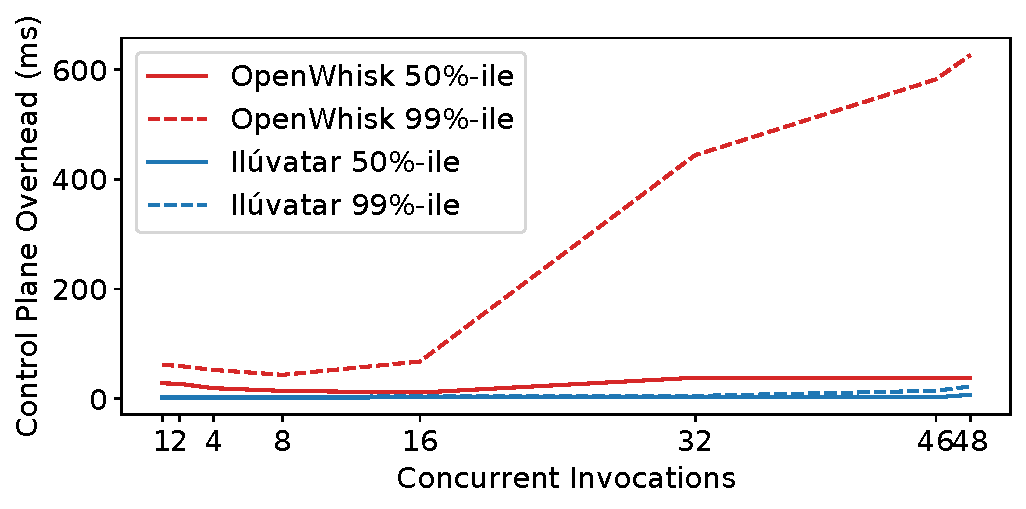
\includegraphics[width=0.4\textwidth]{iluvatar/graphs/scaling/pyaes/overhead-scaling.pdf}
  \caption{The latency overhead of the control plane, as the number of concurrent invocations increases. 
        OpenWhisk overhead is significant and has high variance, resulting in high tail latency. 
        \sysname~ reduces this overhead by 100x. }
  \label{fig:ow-scaling}
\end{figure}


\noindent \textbf{Performance.}
%
Because of its central role in coordinating all aspects of function execution, the control plane plays a major role in determining function performance. 
Managing the function execution lifecycle for hundreds of concurrent invocations imposes a \emph{control plane overhead}, and increases the end-to-end latency.
This control plane overhead can be significant, and affects \emph{all} function invocations, including and especially the ``warm starts''. 
%Time spent in the control plane is simply measured by subtracting the execution time of the function code from the overall end-to-end latency.
This overhead (end-to-end latency minus the function code execution time) for the PyAES function from FunctionBench~\cite{kim2019functionbench} is shown in Figure~\ref{fig:ow-scaling}. 

The figure shows the 50 and 99 percentile overheads as the number of concurrent invocations are increased.
In each case, we are invoking the function repeatedly in a closed-loop, and concurrent invocations are achieved by using multiple client threads.
All invocations are warm starts.
The experiment is run on a 48 core server (more details in Section~\ref{sec:eval}), and the figure thus shows the performance at low and medium load conditions. 

From Figure~\ref{fig:ow-scaling}, we can see that the OpenWhisk latency overhead is more than 10ms,  which is already a significant increase in latency for small functions which dominate real-world FaaS workloads.
Worryingly, the 99 percentile overhead is much higher, and rises to as much as 600ms.
We also see strange inversions in the scaling behavior: the overhead reduces for certain load-levels, and then increases again.
This high overhead, high variance, and uncertain scaling behavior, results in many challenges for FaaS \emph{providers}. 
Due to these issues, low-latency functions see severe performance degradation, and resource provisioning and capacity planning becomes harder due to the high variance and performance unpredictability. 
%

Some of these latency overheads are an artifact of the architecture. 
The shared Kafka function queue can be a major bottleneck; and there are no explicit backpressure or load regulation mechanisms, which is compounded by the CPU overcommitment. 
%
For the sake of comparison, the figure also shows the latency overhead of \sysname~ in the same environment. 
We are able to achieve a per-invocation mean overhead of less than 2ms for almost all the load conditions.
Importantly, the tail overhead is also small: less than 3ms for less than 32 concurrent invocations, rising to 10ms when the system is saturated.


To emphasize, for a median function in the Azure workload which runs for 500 ms, OpenWhisk can increase its latency by 100\%.  
Thus, the control plane plays a crucial role in function performance.
We note that these are the best-case warm-start latencies, when the function's containers is fully initialized and in memory. 
Since function cold-starts impose such a major performance penalty (increasing latency by more than $10\times$), mitigating them has been a major research focus. 
However, because of temporal and spatial locality of access, caching and prefetching techniques can be extremely effective, and the cold-start rate is often less than $1\% $ of all invocations~\cite{faascache-asplos21}. 
The majority of invocations are thus ``warm'', where the performance is dominated by control plane overheads.
%\emph{We thus need a low-latency, low-jitter control plane.}

\noindent \textbf{System Design.}
%
As evidenced by the OpenWhisk architecture presented earlier, FaaS control planes are large, complex distributed systems.
Due to the continually evolving needs of FaaS applications and emergence of new sandboxing techniques (such as lightweight VMs like Firecracker~\cite{firecracker-nsdi20}), they are sandwiched between the scale and heterogeneity of FaaS workloads on one hand, and the deep stack of OS and virtualization components on the other. 

For instance, systems for running web services or microservices do not have to deal with large and highly variable sandbox management overheads, nor with highly heterogeneous request sizes.
For reducing tail latency, these systems can often rely on the OS CPU scheduler for processor sharing, can do CPU allocation at very fine granularity~\cite{kaffes2019shinjuku}, use queuing theory techniques~\cite{prekas2017zygos}, etc. 
At the other extreme, for longer running containers and VMs, their control planes, like OpenStack or Kubernetes face a much lower rate of VM arrivals and departures. and can do careful and ``hard'' resource allocation using bin-packing~\cite{cortez2017resource}.


Functions are highly heterogeneous, and can be seen as both latency-sensitive web requests \emph{and} large containers requiring significant system resources for several seconds. 
FaaS control planes thus have to do \emph{both} low-latency allocation \emph{and} pack CPU and memory resources on their servers carefully to maintain high system utilization.
%
%We posit that these competing needs present new challenges in large-scale distributed resource allocation.
Thus FaaS control planes are one of the more perfect microcosms of challenges in resource management and control in large scale distributed computing. 

A clean-slate control plane design helps us investigate the fundamental performance tradeoffs and challenges in this fast-evolving ecosystem.
Our new implementation also helps to identify the current performance bottlenecks and new avenues of OS optimizations. 


\noindent \textbf{Platform for Experimental Systems Research.}
%
Performance-focused FaaS research is already challenging due to the extreme scale and heterogeneity of the workloads.
These challenges are compounded by existing control planes like OpenWhisk that are unfortunately highly unpredictable.
The control plane jitter and the extreme bimodal cold vs. warm latencies makes it difficult to do reliable and reproducible research~\cite{mytkowicz2009producing}, and subtle environmental and configuration effects can mask the true effects of new research optimizations.
However, it continues to be a key component in developing and evaluating FaaS research~\cite{akkus_sand_2018, shahrad_serverless_2020, faascache-asplos21, faaslb-hpdc22, zhou2022aquatope, ensure-faas-acsos20, alzayat_groundhog_2022}. 
%OpenWhisk is a popular framework which has been used as a platform for investigating and optimizing many facets of FaaS execution.
With OpenWhisk, function performance can be severely affected by a myriad of configuration options, such as insufficient memory for CouchDB, networking configuration, Docker configuration, etc. 

Given the importance of the control plane, we want \emph{predictable} performance to a large degree. 
In our experience, research in FaaS is often hindered by the large overheads and complexity of existing control planes. 
Thus, \sysname~ is designed from the ground-up to be lightweight and provide predictable performance under different conditions. 
Our system implementation can potentially accelerate the development of new optimizations, clarify  our understanding of performance characteristics of this relatively new stack, and provide a platform for robust experiments. 
% Establishing a shared open platform enables easy comparison between research work
With a robust platform, the community can share knowledge and advances, while being able to compare against a well-known and trusted baseline.


\section{\sysname~Design}
\label{sec:design}

% Design goals:
%   A research control plane
%     Easy to use, adjust source code, modification points
%     Full system stack: controller (load balancer), worker(s), load generation, containers, workloads, simulation
%     Configurable, lots of knobs to adjust things easily
%     Tracking of metrics/resources/system events
%   low-variance! and low(ish)-overhead control plane
%   No frivilous features, not too complicated

\sysname's design is guided by our experience of OpenWhisk performance, and by our goals of providing predictable performance, modularity, and a control plane for reliable FaaS research.

% \vspace*{-8pt}
\subsection{Architecture and Overview}
\label{sec:design:arch}

The \sysname~control plane is spread out across a load balancer and the individual workers, and sits above the containerization layers. 
We intend for \sysname~to be the narrow waist~\cite{popa_http_2010} in the FaaS ecosystem: with optimizations for DAG scheduling~\cite{zhou_qos-aware_2022}, state handling~\cite{sreekanti2020cloudburst}, and horizontal scaling~\cite{faaslb-hpdc22} implemented above it, and sandboxing and containerization below it.  
This architecture was motivated by the key question: \emph{Can fast FaaS control planes be implemented with strict layering and separation of concerns?}


We have found that most of the control plane overhead is in the workers, and hence optimizing the worker performance is our major focus.
%
Our architecture is \textbf{worker-centric}, and places more performance and load-management responsibility on the individual workers, instead of a more ``top-down'' centralized approach favored by prior work such as Atoll~\cite{singhvi2021atoll} and others~\cite{kaffes_centralized_2019, kaffes_hermod_2022}.
Top-down resource management requires a consistent global view of the cluster, and is complementary to our work. 
Predictive techniques for load-balancing, prefetching, scheduling, function-sizing can all be effective, but we want to explore the performance characteristics and limits of \emph{reactive} control planes that work with unmodified container runtimes. 

\begin{figure}
  \centering 
  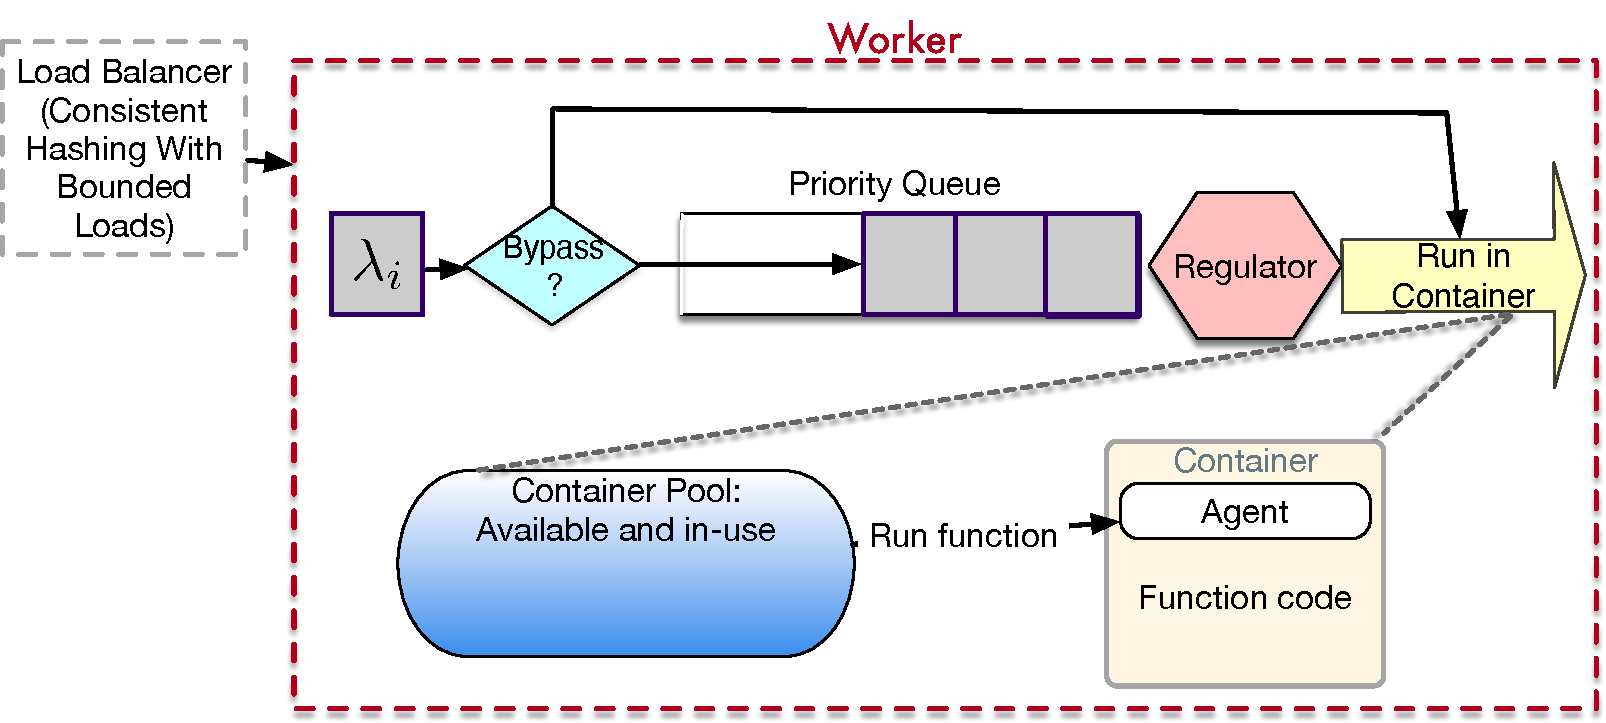
\includegraphics[width=0.95\textwidth]{iluvatar/figs/il76-q.pdf}
    % \vspace*{-6pt}
  \caption{\sysname~has a worker-centric architecture. A per-worker queue helps schedule functions, and regulate load and overcommitment. }
  \label{fig:arch}
  % \vspace*{-6pt}
\end{figure}

\sysname's main components are shown in Figure~\ref{fig:arch}.
Clients/users invoke functions using an HTTP or RPC API, with the main operations being \texttt{register, invoke, async\_invoke, and prewarm}.
Workers also provide load and status information to the load-balancer. 
We use stateless load-balancing, by using variants of consistent hashing with bounded loads (CH-BL), which have been proposed for FaaS recently~\cite{faaslb-hpdc22}. 
This is a locality-aware scheme, which runs functions on the same servers to maximize warm starts, and forwards them to other servers only when the server's load exceeds some pre-specified load-bound.


Continuing on the worker-centric theme, the worker API is a subset and almost completely identical to the overall API, and functions can be launched directly on a worker for single-worker setups and benchmarking, without going through a load-balancer and adding unnecessary latency.
The workers implement various latency-hiding and burst-mitigation techniques. 
All functions are launched inside containers, and dealing with the container layer is a major part of the worker. 
Each worker maintains a container pool of initialized containers for facilitating warm starts, and has an invocation queue for handling dynamic loads.
Function characteristics such as their cold and warm execution times are captured in various data-structures and are made available using APIs for developing data-driven resource management policies.

An important contribution and component of \sysname~is its principled support for function overcommitment based on its queuing architecture.
In many environments, like public FaaS providers, function resources cannot be overcommitted. 
However, the actual function resource usage is often significantly less compared to their requested \quotes{size}.
This difference is the motivation behind recent \quotes{right sizing} work~\cite{akhtar_cose_2020, guo_decomposing_2022, tian_owl_2022, eismann2021sizeless, kotni2021faastlane}, and can significantly improve system utilization.
Through its queue-based architecture, \sysname~supports a wide range of overcommitment scenarios, including no overcommitment, which is absent from OpenWhisk.
By default, OpenWhisk does not overcommit memory, but can  overcommit CPUs, which introduces performance interference and potential SLA violations for functions. 



%%%%%%%%%%%%%%%%%%%%%%%%%%%%%%%%%%%%%%%%


% \subsection{Function handling in the workers}
% \vspace*{-8pt}
\subsection{Function Lifecycle}
\label{sec:design:lifecycle}

%Function lifecycle is controlled by three main \sysname~worker API calls.
New functions first must be \emph{registered}, which entails downloading and preparing its container disk image.
The container images are fetched from DockerHub or some other image repository.
Container images are composed of multiple copy-on-write layers, and we prepare the images by selecting the relevant layers for the operating system and CPU architecture.
The images consist of the user-provided function code and our agent, which is a simple Python HTTP server that runs in each container. 
%How functions are registered and prepared to run by the control plane isn't immediately interesting research-wise, so we choose to do these out-of-band.
%
Registered functions can then be directly \emph{invoked}, which triggers launching of the function's container.
The first invocation is usually a cold start, which entails launching the container image from disk, or from a previous snapshot~\cite{ustiugov2021benchmarking, ao2022faasnap} if available. 
Each function container starts the agent which listens for and controls the actual function code execution. 
The agent has two simple commands, a \texttt{GET /} endpoint for simple status checking, and a \texttt{POST /invoke} to run an invocation with some arguments.
When the container is ready, the worker sends an HTTP request to the agent to start the function code execution. 
We detect the container's readiness using an inotify callback, which is a faster and more generic mechanism for notification compared to Docker's built-in API. 
%
Finally, when the function finishes execution, the HTTP call to the container's agent returns, and the container is marked as \quotes{available} in the container pool, to be potentially used for future invocations of the same function.

\begin{comment}
In the spirit of a fast \quotes{baseline} control plane and for isolation, \sysname~does not share containers across functions.
This is in contrast to SAND's application sandboxing~\cite{akkus_sand_2018}, SOCK's Zygote containers~\cite{oakes_sock_2018}, Nightcore~\cite{jia2021nightcore}, and even OpenFaaS~\cite{openfaas}.
%For example, recently proposed optimizations such as SAND's application sandboxing~\cite{akkus_sand_2018}, or SOCK's Zygote containers~\cite{oakes_sock_2018} share containers for concurrently running functions. 
% allow for functions to share a language runtime inside a container, or the same function to reuse 
% SAND's application sandboxing~\cite{akkus_sand_2018}, or SOCK's Zygote containers~\cite{oakes_sock_2018}. 
%We don't allow concurrent invocations of the same function to run in the same container like OpenFaaS~\cite{openfaas} or nightcore~\cite{jia2021nightcore}.
Our isolation model is similar to the public cloud providers. 
\end{comment}

Additionally, \sysname~introduces a standard \texttt{prewarm}  API call, which starts the function's container and the agent inside of it, and adds it to the container pool.
This reduces most of the cold start overhead associated with the container.
Prewarming can both avoid a \quotes{thundering herd} of cold starts on worker startup, and be an optimization in which the control plane anticipates invocations and prepares containers for them. 
This allows for a systematic mechanism to implement various recently proposed predictive prewarm policies~\cite{roy2022icebreaker, shahrad_serverless_2020, silva_prebaking_2020}. 

%When a container is created, our agent is started up inside it.




\begin{figure}
\centering 
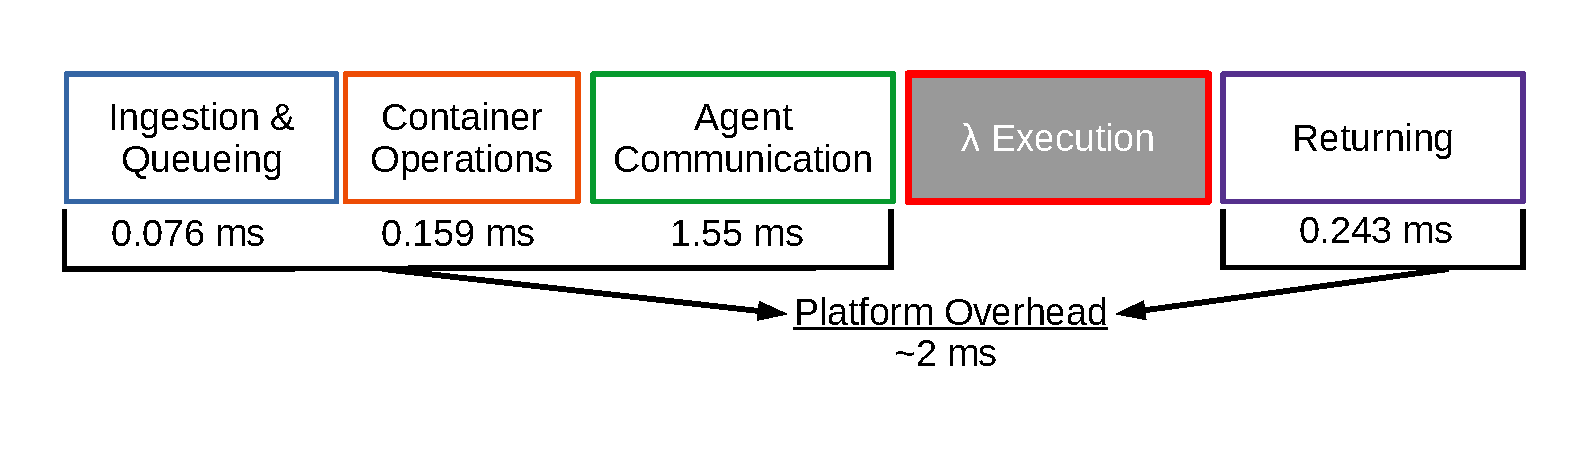
\includegraphics[width=0.95\textwidth]{iluvatar/figs/OverheadTimeline.pdf}
% \vspace*{-12pt}
\caption{The main components of the \sysname~overheads.}
\label{fig:timeline-flow}
  % \vspace*{\myfigspace}
  % \vspace*{-12pt}
\end{figure}


\noindent \textbf{Function Latency Breakdown.}
Throughout \sysname~and this chapter, we are interested in three main performance metrics. 
The first is the end-to-end latency of function execution, also called the \emph{flow time}, shown in Figure~\ref{fig:timeline-flow}.
This in turn has two main components: the control plane overhead is the latency of \sysname~operations, which are mainly before the start of function execution.
The second component is the function execution time, which is determined by the function code, and the load on the system.
The function execution time is our baseline, and we compute the \emph{normalized} end-to-end latency by dividing the full latency by the execution time (also called the \emph{stretch}). 

A more detailed latency breakdown is shown in Table~\ref{tab:overheads}.
The majority of overhead comes from the communication with the agent which is over HTTP. 
This is a deliberate choice, since we wanted to be compatible with existing OpenWhisk function images.
This can be reduced by using faster IPC mechanisms like in Nightcore~\cite{jia2021nightcore}. 
However, these faster communication approaches would reduce compatibility, especially with functions deployed inside VMs.

For OpenWhisk, a similar latency breakdown shows that a large amount of time is spent reading/writing to CouchDB (up to half a second), and the rest of the slowdown occurs in the Invoker (OpenWhisk's worker) and is primarily due to its design and implementation. 
Interestingly, the load-balancer/controller for OpenWhisk adds less than 3ms of latency even under heavy load, indicating that the worker-level performance is relatively more important. 
This further motivates our worker-centric design and evaluation focus. 


\begin{table}
  \centering 
  \caption{Latency of different \sysname~worker components for a single warm invocation.}
  \label{tab:overheads}
  \begin{tabular}{|c|c|r|}
    \hline
    Group & Function Name & Time (ms) \\
    \hline
    Ingestion \& Queuing & \begin{tabular}{@{}c@{}}invoke \\ sync\_invoke \\ enqueue\_invocation \\ add\_item\_to\_q \end{tabular} & \begin{tabular}{@{}c@{}}0.026 \\ 0.013 \\ 0.017 \\ 0.02 \end{tabular} \\
    \hline
    Container Operations & \begin{tabular}{@{}c@{}}spawn\_worker \\ dequeue \\ acquire\_container \\ try\_lock\_container \\ \end{tabular} & \begin{tabular}{@{}c@{}}0.029 \\ 0.02 \\ 0.096 \\ 0.014 \\ \end{tabular} \\
    \hline
    Agent Communication & \begin{tabular}{@{}c@{}}prepare\_invoke \\ call\_container \\ download\_result \\ \end{tabular} & \begin{tabular}{@{}c@{}}0.154 \\ 1.364 \\ 0.032 \\ \end{tabular} \\
    \hline
    Returning & \begin{tabular}{@{}c@{}}return\_container \\ return\_results \\ \end{tabular} & \begin{tabular}{@{}c@{}}0.017 \\ 0.266 \\ \end{tabular} \\
    \hline
  \end{tabular}
\end{table}

%As we can see, the overheads are minimal. Some queuing, some agent communication, which totals to about 3ms. 
% \vspace*{-8pt}
\subsection{Worker Performance Optimizations}
\label{sec:design:worker}

To achieve this low latency function execution for heterogeneous and bursty workloads, \sysname~uses two key underlying design principles: resource caching, and asynchronous handling of function life-cycle events.

\subsubsection{Resource Caching}

The cornerstone design goal of \sysname~is to reduce jitter, which we accomplish by removing expensive operations from the function's critical path. 
Instead, we cache and reuse as many function resources as possible, which minimizes the \quotes{hot path} function invocation latency significantly.
This principle is applied in various worker components, which we describe below.
A fast \textbf{Container Pool Keep-alive} and cached \textbf{HTTP Clients} allow for efficient warm start invocations.
Pre-allocating and caching \textbf{Network Namespaces} shortens cold starts---a technique first used for rapid container provisioning~\cite{oakes_sock_2018};

\noindent \textbf{Container Keep-alive.}
The primary and exemplary application of resource caching is in the container keep-alive cache that \sysname~workers maintain.
The containers become \quotes{warm} when their function has finished execution, and become \quotes{available} for the next invocation of the same function. 
We maintain a pool of all in-use and available containers for each registered function.
This container cache implements classic eviction policies such as Least Recently Used (LRU), and size-aware policies like Greedy-Dual-Size-Frequency, as proposed in FaasCache~\cite{faascache-asplos21}. 

\noindent \textbf{Network Namespace Caching.}
For isolation, each container is provided with a virtual network interface and a network namespace.
Through performance profiling, we've found that creating this network namespace can add significant latency to container cold starts---as much as 100ms.
This is due to contention on a single global lock shared across all network namespaces~\cite{oakes_sock_2018}. 
To minimze this overhead, we maintain a pool of pre-created network namespaces that are assigned during container creation. 
The isolation is still maintained, since concurrently running containers do not share the namespace. 
%Avoiding this expensive operation on the critical path.

\noindent \textbf{HTTP Clients.}
The worker threads communicate with the in-container agent for launching the function code.
Instead of creating a new HTTP client for every invocation, we cache a client per container and use connection pooling. 
This affects all invocations (even warm starts), and reduces the control-plane overhead latency by up to $3ms$. 

\subsubsection{Async Function Life-Cycle Handling}

The second key design principle is to handle various aspects of the function's lifecycle asynchronously off the critical path.
\sysname~achieves this through background worker threads for certain tasks, and through its Rust implementation which heavily uses asynchronous functions, futures, and callbacks wherever possible. 

\noindent \textbf{Keep-alive eviction.}
One such aspect is maintaining the function keep-alive cache, and ensuring that new functions have enough free memory to launch without waiting on existing containers to be evicted first.
Traditionally, eviction decisions would be made in an online fashion, but picking victims and waiting for their removal creates high variance in function execution times. 
\sysname~performs container eviction from the keep-alive pool  periodically in the background, off the critical path. 
This is similar to the Linux kernel page-cache implementation. 
We maintain a minimum free-memory buffer for dealing with invocation bursts, and periodically sort the containers list for eviction based on caching policies from~\cite{faascache-asplos21}. 

\noindent \textbf{Function Queuing.}
An important component of \sysname's architecture is a per-worker function queue.
New invocations are first put into the queue, and are dispatched to the container backend by a queue monitoring thread. 
%only when sufficient resources are available.
This allows us to tolerate bursts of invocations, and regulate the server load. 
% Details of our queuing policies are presented in Section~\ref{sec:q}.

%%%%%%%%%%%%%%%%%%%%%%%%%%%%%%
% \vspace*{-8pt}
\subsection{Container Handling}
\label{sec:design:ctr}

\sysname~uses standard Linux containers for isolating and sandboxing function execution---a \quotes{vanilla} and conventional approach.  
Several exciting new isolation mechanisms for cloud functions
have been proposed: such as lightweight VMs~\cite{firecracker-nsdi20}, unikernels, WASM~\cite{shillaker2020faasm} and other language runtimes~\cite{graalvm}, etc. 
Importantly, the sandboxing affects the \emph{cold start} overheads, which account for a tiny fraction of all invocations (usually less than 1\%).
Our control plane design and performance optimizations are independent of the sandboxing mechanism, and we address the orthogonal problem of optimizing the \emph{warm starts}. 

The basic container operations we use are: i) Create a container/sandbox with specified resource limits and disk image/snapshot, ii) launch a task inside it for the agent, and iii) destroy the container.
Each container is launched with the CPU and memory resource limits. CPU limits are enforced with cgroup quotas. 
This limited API allows \sysname~to support \emph{multiple} container backends.


By default, we use containerd~\cite{containerd}, which is popular container library, also used by Docker. 
The very rich containerization ecosystem presents a large number of options, and examining their tradeoffs was a major part of \sysname's design process.
Importantly, the choice of containerization library impacts the cold start times, and some library operations can take considerable time (100s of ms). 
High-level container frameworks like Docker are feature-rich and easy to use, but are typically used for long-running containers and are not optimized for latency.
Docker uses containerd under the hood, and it provides  more fine-grained control and slightly better latency.
Functions require a minimal containerization, and a lot of feature-complexity in these large containerization libraries can add to latency.
For instance, the crun~\cite{crun} library which is written in C takes about 150ms to launch a container, whereas containerd (written in Go) needs 300ms, and Docker needs 400ms. 

Using containerd allows us to use the OCI container specification~\cite{oci}, and makes it easier to support other container runtimes.
For instance, we also support the Docker container backend, which required only a minimal programming effort.
Containerd operates as a separate service, and we use it's RPC-based API, which contributes to some latency as well.
We contemplated writing our own optimized container runtime in Rust to avoid the overheads due to inter-process communication, extra process forks and system calls, and implement other cgroups and namespace optimizations. 
However, we ended up going with containerd to keep our control plane small and reusable across container runtimes.
We also wanted to investigate and tackle the challenge of getting predictable performance out of higher level containerization services that are not part of the same address space. 


\noindent \textbf{Simulation Backend.}
In addition to containerd and Docker containers, we also support a \quotes{null} container backend which is useful for simulations and evaluating control plane scalability.
%
Because of the scale and variety of FaaS workloads, using discrete event simulators for developing and evaluating resource management policies is often necessary.
%
For instance, the recent work on FaaS load balancing~\cite{faaslb-hpdc22} uses such a simulator for evaluating their policies at scale for different subsets of the Azure workload trace.
Usually, the simulation is used to augment and complement the \quotes{real} empirical evaluation of the same policies which are implemented in FaaS frameworks like OpenWhisk. 

However, a major methodological and practical issue is that the policy implementations, workload generation, and analysis, all need to be duplicated across the simulator and the real system.
This can lead to subtle and large divergences between the simulation and real environment. 
Moreover, the simulator cannot capture all the real-world dynamics and jitter, and can suffer from poor fidelity.

In order to aid researchers, \sysname~takes a different approach to simulations, and provides \emph{in-situ} simulations. 
Our \quotes{null} container backend does not run any actual function code, but instead sleeps for the function's anticipated execution time.
The rest of the control plane operates exactly as with real containers, and we still handle all other aspects of the function's lifecycle.
%
This allows us to simulate large systems and workloads. 
For evaluating any particular policy, researchers can use the simulator null-backend to evaluate control-plane overheads, warm-starts, etc., without requiring a large cluster.
Each \sysname~worker can \quotes{simulate} 100s of cores, since the CPU resources are only being consumed by the control plane, and not for running actual functions.
Alternatively, a large cluster can be simulated with multiple simulated workers. 

With this approach, \emph{there is minimal difference} between the simulation and the real system. 
Thus an experiment can be run in-situ or in-silico, following identical code paths.
The main distinction is that API calls to containerd are replaced with internal dummy function calls, and function invocations are converted to sleep statements.  
All control plane operations, control-flow, logging, resource limits enforcement, etc., are exactly the same as with the \quotes{real} \sysname.
This also helps with mocking and testing new policies. 

%%%%%%%%%%%%%%%%%%%%%%%%%


%%% Local Variables:
%%% mode: latex
%%% TeX-master: "paper"
%%% End:


\section{Function Invocation Queuing}
\label{sec:q}

As a way to regulate and control function execution and worker load, \sysname~ incorporates a per-worker invocation queue architecture. 
Function invocations go through this queuing system before reaching the container manager, which either locates the warm container and runs the function or creates a new container.
Each worker manages its own queue, differentiating our design from OpenWhisk's shared Kafka queue. 

\noindent \textbf{Motivation.}
%
This queuing architecture is motivated by three main factors: i) the bursty nature of the workload , and ii) Reducing cold starts due to concurrent invocations, and iii) to give workers additional mechanisms for controlling their load, implementing prioritization, etc. 
Note that once the function passes through the queue, it is effectively ``scheduled'' for execution by the OS CPU scheduler.
The CPU scheduler of course has its own throttling and controling mechanisms, such as cgroups and the various scheduler tuning knobs.
The invocation queue thus acts as a kind of a regulator or a filter before the CPU scheduler, and ideally, ``feeds'' it the right functions at the right rates for maximizing throughput and minimizing latency.
%

Because function workloads are so bursty and heterogeneous, running each function immediately can significantly increase the worker load and result in severe resource contention and increase  function tail latencies.
%
The queue also helps as an explicit back-pressure mechanism for load-balancing, admission control, and elastic scaling.
The queue length is  used for accurately determining the true load on the worker, which is a vital input to consistent hashing with bounded loads~\cite{faaslb-hpdc22}.
This reduces the staleness and noise of using system load average as the load indicator, and makes load balancing more robust.


Queuing invocations also allows us to reduce cold-starts.
While repeated function invocations are good and increase warm starts, 
\emph{concurrent} invocations of the same function results in cold-starts for all the concurrent invocations, since each invocation needs to be run in its own container.
This is also the ``spawn start''~\cite{ristov_colder_warmer}, which causes severe latency increase of 10s of  seconds in public FaaS. 
If there are $n$ concurrent invocations that arrive at the same time, then the $n$ concurrent cold-starts can significantly increase the system load and affect latency of other functions.
Instead, by queuing and throttling the functions, we can wait for the invocation to finish, and then use the warm container for the next function in this ``herd'', and so on and so forth. % Lol zizek 
%Having a queue allows us to regulate the invocations by this and other means. (?) 

% \vspace*{-8pt}
\subsection{Queue Architecture}
\label{sec:q:arch}

\sysname's queue architecture is shown in Figure~\ref{fig:arch}.
We have three main components.
%
From right to left, first, we have a concurrency regulator (or just regulator), which enforces the \textbf{concurrency limit}: the  upper-bound on the number of concurrently running functions. 
%
This lets functions execute \quotes{on cpu} without timesharing, and effectively determines the overcommitment ratio.
Higher concurrency limits (more than the number of CPUs) means  more CPU overcommitment.
Note that even with overcommitment, the cgroup quotas still provide proportional allocation (thus a 2 CPU container will still get twice the CPU cycles compared to a 1 CPU container). 
%
In addition to concurrency, other factors can also be used to regulate the queue discharge rate. 
The regulator can be used to run functions of only when sufficient resources (such as CPU bandwidth, warm containers, or even accelerators like GPUs) are available. 


%Note that technically the queue service backend is a processor sharing system, so can tolerate immediate execution albiet under heavy load.
%The concurrent cold start mitigation is one important component of the regulator policy.
%Its inputs are the number of currently running functions, the state of the container map to see which functions are executing, and the system resource utilization (load average, cpu\%, etc).
%This allows custom policies: we may want to limit the load average to under some limit, or the number of functions ``in flight'', etc.
\sysname~can be deployed with a fixed concurrency limit based on the usage requirements, or use its dynamic concurrency limit mode. 
In the dynamic mode, we use a simple TCP-like AIMD~\cite{yang2000general} policy which increases the concurrency limit until we hit congestion, which in our case is hit if the system load average increases above some specified threshold. 
Other metrics are possible: looking at the increase in execution time (i.e., stretch) of the functions could also be used as a congestion metric.
The concurrency limit affects the tail-latency, and more advanced policies can be implemented. 


\begin{comment}
Having the container map also allows us to implement \textbf{concurrent cold-start mitigation}.
If the function at the head of the queue has no warm containers available, and one of its instantiations is running, then we put the function back in the queue.
As a function's warm start is typically orders of magnitude shorter than cold starts, it is better for it to wait for warm container than to cold start one.
We implement this by asking the container pool for a warm container, and if it fails to give us one we can re-queue the invocation for the future.
Optionally, we can allow for a cold start to increase the number of warm containers for a function, naturally scaling if there is an increase in frequency.
\end{comment}

% This is currently implemented by looking at the container pool and estimating the likelihood of a warm vs. cold start, and using that expected execution time.
% The number of current concurrent executions are stored in the system statemap.


The second component is a \textbf{queuing discipline.} 
In the simplest case, we can use simple FCFS, and process functions in arrival order.
However, because functions are heterogeneous, this is not always the most appropriate.
Instead, we can use the past function execution characteristics such as their cold/warm running times for size-aware queuing such as shortest job first (SJF).
We elaborate more on the queuing policies in the next subsection. 

Finally, we note that queuing may increase the waiting time for small functions.
We thus have a \textbf{queue bypass} mechanism, which allows certain functions to bypass the queue and immediately and directly run on the CPU. 
Bypass policies take the function running time and the current system state as input. 
Currently, we implement a short-function bypass, where functions smaller than a certain duration are immediately scheduled, as long as the system is under a load-average limit.  
More effective bypass policies can also consider reinforcement learning approaches, since the action space is simple (bypass or enqueue), and the system state is well defined (functions running and in-queue, etc.).


% \vspace*{-8pt}
\subsection{Queuing Policies}
\label{sec:q:pol}

We implement multiple queue policies which leverage the repeated invocations of functions and use their learned execution characteristics to determining each function's priority.
To accomplish this, we maintain per-function characteristics such as cold time, warm time, and inter-arrival-time (IAT). 
%We maintain a sorted priority queue of invocations. 
We maintain a priority queue sorted by the function priorities, which are computed using their characteristics like arrival and execution time. 
%We can priority calculation to yeild differnt policy results.
%Different priority calculation yields different priorities. 

FIFO is simplest and invocations are just sorted by their arrival time.
For prioritizing small functions, we leverage our bypass mechanism, where the short functions can skip the queue and be scheduled directly on the CPU. 
Optimizing queuing policies for heterogeneous functions is challenging, and is an NP complete problem even in the offline case~\cite{bender1998flow}.


For improving throughput, we use shortest job first (SJF), which helps reduce the waiting time for short functions, but can lead to starvation for longer functions if the queue never drains. 
As a tradeoff between function duration and arrival, \sysname~ by default tries to minimize the ``effective deadline'' of a function, which is equal to the sum of its arrival time and (expected) execution time.
This earliest effective deadline first (EEDF) approach balances both short functions and starvation.
In both SJF and EEDF, an invocations' execution time is determined by its (moving window) warm time.
New/unseen functions have their times set to 0, to prioritize their execution.  
If we expect to find available containers for a function, we use its (moving window) warm time as the execution time in both SJF and EEDF.
Otherwise, we use its cold time---this also helps in reducing the concurrent cold starts, since the expected cold invocations of some functions in a burst separates them in the queue, and reduces the number of concurrently executing identical functions.
This spreading of function invocations over time increases the warm starts and overall performance. 
%
%Finally, we can  also prioritize functions with the highest inter-arrival-time. 
Finally, the RARE policy prioritizes the most unexpected functions (i.e., functions with the highest IAT). 

%All these policies can be combined with the short-function bypass technique.
%This also reduces the queue size and thus the overheads associated with maintaining a priority queue.
%In practice, the concurrency limit is larger than the number of the CPUs, so the queuing is expected to minimal under steady-state conditions. 


%L-p fairness:  $(\sum F^p)^{1/p}$


%%% Local Variables:
%%% mode: latex
%%% TeX-master: "paper"
%%% End:


\section{Implementation}
\label{sec:impl}

% Use a lot of provided stuff as a starting point
%   Containerd for isolation/container startup
%   CNI for networking
%   prebuilt Docker images
%   Rust language for efficient compiled language, without garbage collection interference
%   Tokio async handling & userspace threads

\sysname~ is implemented in Rust in about 13,000 lines of code.
It will be open-sourced upon paper acceptance. 
Its low latency and lack of jitter are attributable to the various low-level profile-guided performance optimizations we have implemented during the course of its development and testing.
Function handling and container management in the worker make up a majority of the implementation footprint and focus. 
Ours is a heavily asynchronous implementation using the \texttt{tokio} library in Rust, and various function lifecycle events spawn new userspace threads and trigger callbacks. 
The major data structure shared by the various worker threads is the container pool, which is implemented using the \texttt{dashmap} crate, which is a concurrent associative hashmap--- this provides noticeable latency improvements compared to a mutex or read-write lock.
Conversely, we still use a mutex for the queue, since we found minimal performance degradation compared to a no-queue architecture during profiling. 
These, and many other small optimizations, keep the \sysname~
resource consumption small: even under a heavy and sustained load that saturates a 48 CPU server, the worker process uses less than 20\% of a single CPU core. 




%%%%%%%%%%%%%%%%%%%%%%%%%%%%%%

%\noindent \textbf{Agent Optimization.}
%All our functions are written Python, and we do some Python-specific optimizations during their prewarm.
%The agent imports the function Python code, loading it and any library dependencies into memory, plus executing statements not in functinos, such as downloading an ML model.


% \paragraph{Deployment}
% For ease of repeatable and scalable use, we have set up our system to be deployable with Ansible \cite{}.
% In a command it can configure, set up, and tear down the applications that make up \sysname{}, and even capture artifacts like logs.
% It ties in nicely with the detailed configuration supported by our worker and controller services.
% Our services support configuration via a json file, convenient for development and local testing, but less so for large research experiments.
% Ansible, plus some clever config loading, allow us to inject arbitrary values as part of a larger command, making deployment for different experiments a breeze.

% With this setup, \sysname{} can be configured and deployed to any number of nodes with a single command.
% With this we easily scripted a variety of setups for our experiments in Section \ref{Evaluation}, giving us consistent and controlled environments and results.
% Workers are configured with a json file on startup, with the various policy options (such as queuing), keep-alive, timeouts, networking, logging, etc.

% CNI and container-spec are also provided as json files. For the container-spec, we change....

% Workers have four main services: Containers, invocation, network, and status.

% \vspace*{-8pt}
\subsection{Support for FaaS research}
\label{sec:impl:support}

One of our major design goals is for a reliable and extensible control plane for performance-focused FaaS research.
We now describe some of the \sysname~ features and our experiences in extending it.


\noindent \textbf{Performance Metrics.}
We keep track of all internal and external function metrics (such as their cold/warm execution time histories, inter arrival times, memory footprints, etc.) and provide them to all components of the control plane, and also to external services.
%
One of \sysname's implementation goals was to reduce the reliance on external services for system monitoring etc.
We thus track key system metrics like CPU usage, load averages, and even CPU performance counters and system energy usage using RAPL and external power meters.
These metrics are collected using async worker threads, and provide a single consistent view of the system performance.
%
Additionally, we also use and provide Rust-function tracing for fine-grained performance logging and analysis.
We use the \texttt{tracing} crate to instrument the passage of invocations through the control plane components, and obtain detailed function level timing information, which is used for identifying control plane and container-layer bottlenecks. 
%These logged details helped us with performance bottlenecks, but by default we keep disabled because it can increase per-invocation latency due to the overheads and CPU contention from creating so many logging events and it increases log file output size dramatically. 

\noindent \textbf{Adding New Policies and Backends.}
%
Using function and system metrics allows for easy development of data and statistical learning based resource management policies to be implemented.
Our baseline policy implementations for keep-alive eviction, queuing, load-balancing, are all easily extensible using Rust traits, polymorphism, and code generation. 
In our experience, adding new policies is relatively straight-forward, even for new-comers.
For example, all the priority-based queuing policies (SJF, EEDF, RARE, etc.) were implemented by extending the base FCFS policy.
Implementing and testing these policies took less than a few dozen lines and about four hours for a graduate student unfamiliar with the code-base. 

The default container runtime backend is \texttt{containerd}, but the interface is small, and supporting new backends is relatively easy.
We added Docker support in about 400 lines and one person-day of development effort.


\textbf{Load-generation and Testing.}
In the spirit of providing a full-featured system for FaaS experimentation, we have developed a load-generation framework.
It can do closed and open loop load generation, and be parameterized by the number and mixture of functions, their IAT distributions, etc. 
The testing framework can use functions from FaaS suites like FunctionBench~\cite{kim2019functionbench}, or custom sized functions that run lookbusy~\cite{lookbusy} for generating specific CPU and memory load.
%
The open-loop generation produces a timeseries of function invocations, which is helpful for repeatable experiments.
The functions' IAT distributions can be exponential, or be derived from empirical FaaS traces like the Azure trace~\cite{shahrad_serverless_2020}.


For the Azure trace, we start by randomly sampling functions and computing the CDF of their IATs.
We compute the expected load level in the system using Little's law, by finding the expected number of concurrent invocations for each function and adding them for all functions.
This expected load can be significantly different from the capabilities of the system under testing (for example, 100 concurrent functions will overload a 12 core system). 
Therefore, we can scale the individual function IAT CDFs to find a suitable load. This also allows us to change the relative popularities of individual functions, and conduct fine-grained sensitivity experimentation (like examining system performance when the popularity of one single function
changes, etc.).
We can generate larger traces by layering, and merging the traces from multiple smaller workloads.  


For synthetic functions (using lookbusy), we use their distribution of running times and memory consumption when generating the workload.
When using real functions from a benchmark-suite like FunctionBench, for each randomly sampled function, we use its average execution time (from the full trace), and assign it the closest function in the suite.
For example, if the average running time of a candidate function in the Azure trace is 8 seconds, we represent it using the ML-training function, which has the closest running time of 6 seconds.




%%%%%%%%%%%%%%%%%%%%%%%%%%%%%%


%%% Local Variables:
%%% mode: latex
%%% TeX-master: "paper"
%%% End:


\section{Experimental Evaluation}
\label{sec:ilu:eval}
We have extensively tested \sysname's performance characteristics throughout its development.
Here, we present a limited set of its key performance attributes and focus on new insights into FaaS performance.
All our experiments are conducted on a 48 core Intel Xeon platinum 8160 CPU, and we restrict the worker to 32 GB memory, running Ubuntu 20.04 using Rust version 1.67.0 and Tokio library version 1.19.2.
%
We are interested in evaluating latency overheads and \sysname's suitability as a low-jitter research control plane. 
This evaluation focuses exclusively on the performance of the worker, where we think most per-invocation latency improvement opportunities exist.
Many effective load-balancing policies have been published, but their impact on latency is limited to balancing decision time and warm start ratio.
Our stateless controller's overhead is consistent at less than 0.5ms, and we can thus ignore its latency contribution, for ease of exposition.
Our CH-BL based load-balancer maximizes locality and provides 99\% warm starts, and we focus on single-worker performance to remove unnecessary confounding factors.

% \noindent \textbf{Load Generation.}
% To collect benchmarking data and testing Control Plane Overhead for the different functions we generate \emph{closed loop} requests with varying client threads for 30 min each. We calculate the average for normalization of data collected in any other experiment. 

% For testing different Queue Policies we use open loop request generation. 

% \noindent \textbf{System Tweaks.}
% Ilúvatar itself keeps track of the memory usage and can limit number of concurrent requests dispatched to the system. We use Linux CPU Hotplug support to turn off some of the CPU cores to limit the system size. 

% \vspace*{-8pt}
\subsection{Control Plane and Function Performance}
\label{sec:ilu:eval:ovhead}

\begin{figure}
  \centering  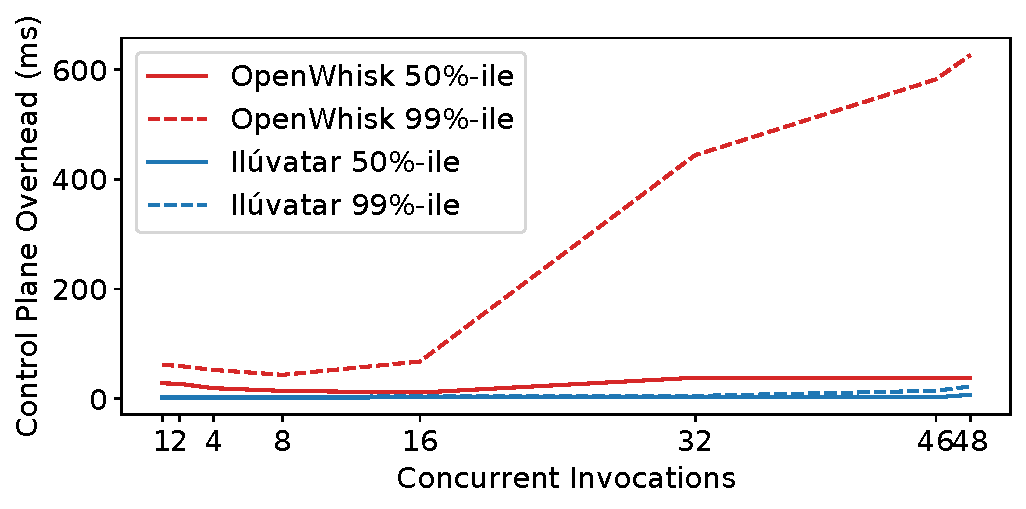
\includegraphics[width=0.6\textwidth]{iluvatar/graphs/scaling/pyaes/overhead-scaling.pdf}
  \caption{The latency overhead of the control plane, as the number of concurrent invocations increases. 
        OpenWhisk overhead is significant and has high variance, resulting in high tail latency. 
        \sysname~reduces this overhead by 100x. }
  \label{fig:ow-scaling}
\end{figure}

\begin{comment}
\begin{figure}
    % Results for pyaes, which has runtime of ~300 ms
    % [0.8, 0.9, 0.99, 0.999, 0.9999, 0.9999]
    % 1 [2.26 2.29 2.40 4.40 4.59 4.59]
    % 2 [2.19 2.24 2.32 3.97 4.74 4.74]
    % 4 [2.28 2.32 3.07 4.81 5.76 5.76]
    % 8 [2.27 2.31 2.48 4.84 12.16 12.16]
    % 16 [2.60 3.02 4.65 7.89 8.66 8.66]
    % 32 [3.18 3.36 4.97 7.91 10.71 10.71]
    % 46 [5.02 6.19 14.50 20.25 26.02 26.02]
    % 48 [12.31 14.89 22.25 28.86 32.52 32.52]
  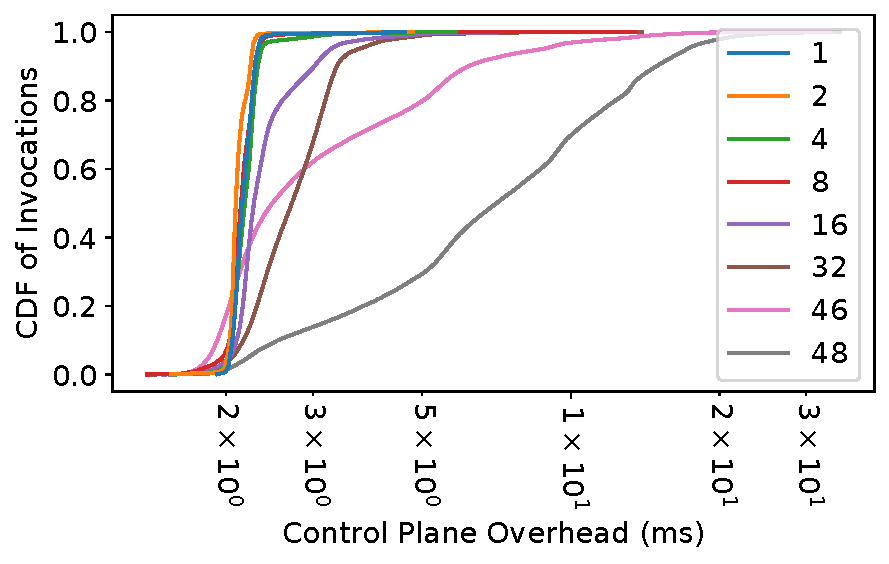
\includegraphics[width=0.6\textwidth]{iluvatar/graphs/scaling/pyaes/overhead-cdf.pdf}
    %  \vspace*{-6pt}
     \caption{\sysname~provides low latency overhead across a range of concurrent invocations.}
        % \vspace*{-6pt}
    \label{fig:ovh-cdf-aes}
\end{figure}
\end{comment}
% Results for lin_pack which has runtime of ~300 microseconds
% Percentiles: [0.8, 0.9, 0.99, 0.999, 0.9999, 0.9999]
% Thread count results (in milliseconds):
% 1 [2.69 3.01 5.68 940.41 956.48 956.48]
% 2 [2.69 2.94 7.12 940.17 942.17 942.17]
% 4 [2.16 2.53 5.74 928.90 935.37 935.37]
% 8 [2.00 2.35 4.78 833.26 860.58 860.58]
% 16 [3.13 3.70 7.05 664.69 709.56 709.56]
% 32 [6.30 7.54 13.78 351.35 430.77 430.77]
% 46 [9.62 11.83 20.14 103.92 15406.05 15406.05]
% 48 [9.64 12.14 20.85 73.48 31507.97 31507.97]

% Results for json_dumps_loads which has runtime of 0.5-1.5 seconds
% [0.8, 0.9, 0.99, 0.999, 0.9999, 0.9999]
% 1 [3.41 3.50 3.87 7.66 10.54 10.54]
% 2 [3.41 3.48 3.99 7.09 12.99 12.99]
% 4 [3.61 3.70 4.20 7.93 8.59 8.59]
% 8 [3.74 3.85 4.81 9.00 15.24 15.24]
% 16 [3.73 3.85 4.27 8.35 15.27 15.27]
% 32 [4.08 4.21 5.15 8.77 15.98 15.98]
% 46 [4.10 4.24 5.27 8.95 15.92 15.92]
% 48 [4.11 4.25 5.17 8.79 16.02 16.02]  

In this subsection, we focus on the latency overheads of \sysname~under different workloads and configurations.
For these experiments, we do not use any queuing, use a single worker, and focus on the most basic \sysname~configuration.  

We start by examining the control plane overheads under a closed-loop load for 30 minutes generated by different number of client threads. 
The control plane overhead CDF for the AES function is shown in Figure~\ref{fig:ow-scaling}. %~\ref{fig:ovh-cdf-aes} 
With 48 concurrent client threads, all the CPUs are fully utilized by function execution. 
Even in this saturated case, the 90 percentile overhead is less than 20ms. 
Just below this saturation limit, with 46 threads, the 90 percentile overhead drops to less than 10ms, and the average is less than 3ms. 

%%%%%%%%%%

\begin{figure*}
  \centering
  \subfloat[PyAES \label{fig:flow:pyaes}] {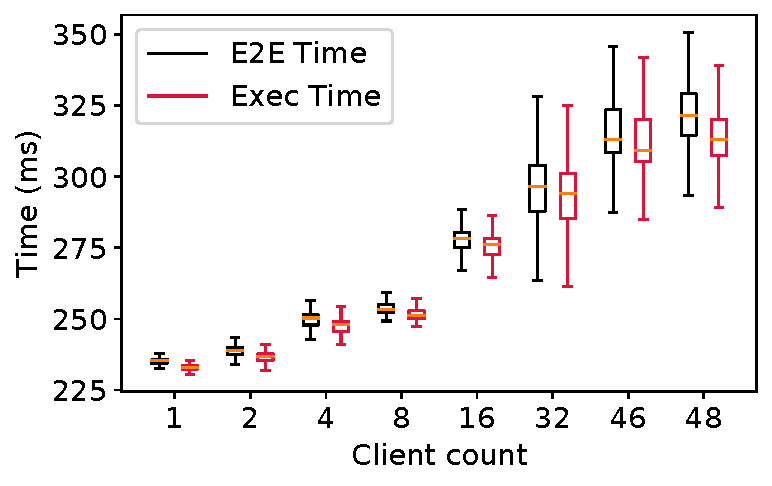
\includegraphics[width=0.3\textwidth]{iluvatar/graphs/scaling/pyaes/worker-e2e-and-exec.pdf}}
    \subfloat[JSON \label{fig:flow:json}] {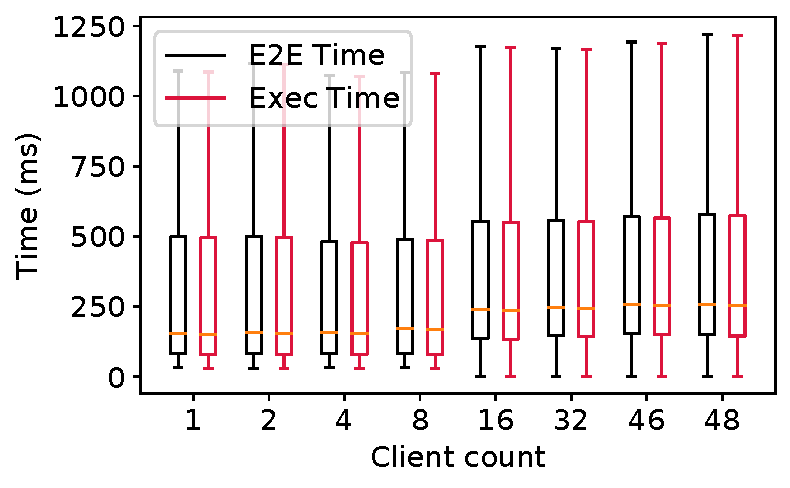
\includegraphics[width=0.3\textwidth]{iluvatar/graphs/scaling/json_dumps_loads/worker-e2e-and-exec.pdf}}
    \subfloat[Video \label{fig:flow:video}] {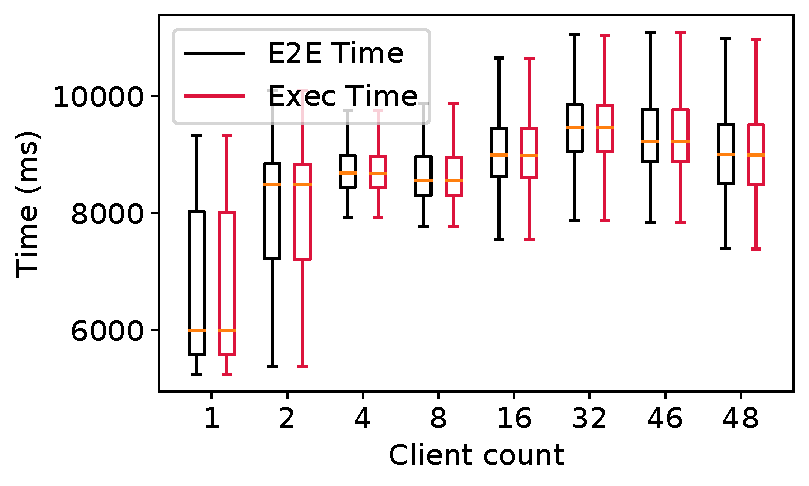
\includegraphics[width=0.3\textwidth]{iluvatar/graphs/scaling/video_processing/worker-e2e-and-exec.pdf}}
      %  \vspace*{-6pt}
      \caption{End-to-end latency and execution times for different functions as we increase the concurrency levels.}
        %  \vspace*{-6pt}
  \label{fig:flow-fn-all}
\end{figure*}

We now provide a more detailed breakdown of the function latency.  
In Figure~\ref{fig:flow-fn-all}, we look at the end to end (E2E) function latency (i.e., flow time) and execution time of different representative functions under different loads.
The flow time is impacted by the control plane overhead and the function code execution time. 
Both these factors are affected by the system load, which in turn is affected by the concurrency level.
% We vary the number of clients invoking the same code in a closed loop, and had each client register the code as a unique function with the system.
The difference between the E2E and the function execution time is the control plane overhead, which is small for all functions and at all load levels.


Interestingly, a significant source of latency variance is the function execution time itself. 
For the small, CPU-intensive PyAES function (Figure~\ref{fig:flow:pyaes}), the  inter-quartile-range is 60ms, which is 20\% the average execution time.
Both the execution time (and hence the E2E latency) and the variance also increases with the system load.
%
This variance is also determined by the non-determinism in the function code.
For instance, the JSON function (Figure~\ref{fig:flow:json}) parses a random json file on every invocation, and thus has a higher natural variance in its execution time.
%
Finally, the video processing function is long and CPU intensive: it downloads and converts a video to grayscale. 
This magnifies the CPU contention, and the function latency increases from 6 to 9 seconds under heavy load.
%


The notable increase in execution time for all three functions is a result of  high  CPU cache miss percentage and a reduction in the instructions per cycle (IPC).
%
We also observed poor cache locality with an increasing number of CPU cores. When the same workload was run on half the number of CPUs (by disabling the rest of the CPU cores), the cache miss percentage significantly dropped (by more than 50\%), along with a proportionate reduction in the latency variance.
%
This highlights and emphasizes the deeper architectural challenges of FaaS, which were also shown by~\cite{shahrad_architectural_2019}. 
%We leave the study of the cause of this effect for future work.

\noindent \textbf{Result:} \emph{\sysname~overheads are small even under heavy load. Function code non-determinism and system load have a higher impact on the function execution times. }


%%%%%%%%%%%%%%%%%%%%

\begin{figure}
  \centering
  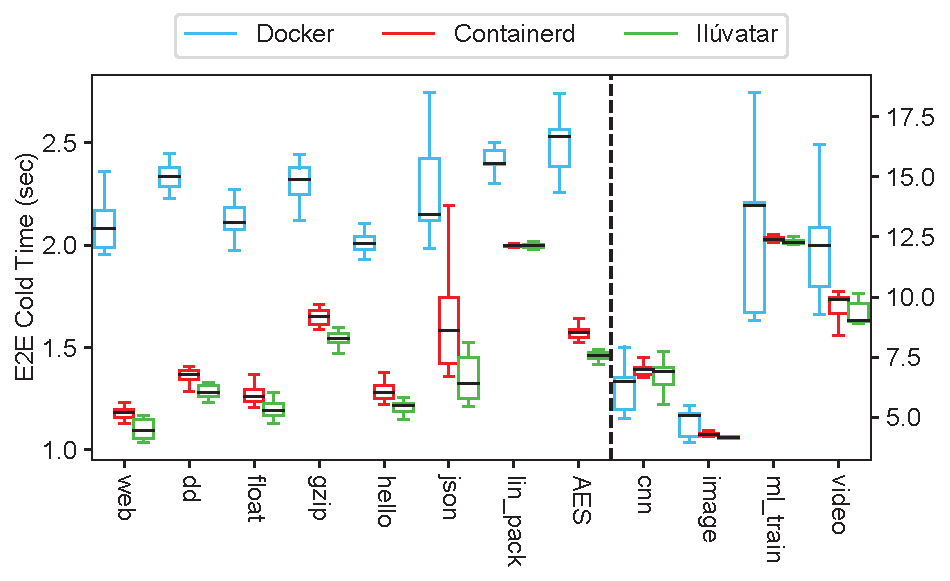
\includegraphics[width=0.6\textwidth]{iluvatar/graphs/impl/benchmark_cold_e2e.pdf}
  % \vspace*{-6pt}
  \caption{Most functions benefit from using a lower-level containerization and OS object caching on cold starts.}
  \label{fig:cold}
  % \vspace*{-6pt}  
\end{figure}

\noindent \textbf{Cold starts.}
So far, we have focused on warm-start performance which dominates function workloads.
\sysname~also incorporates a few optimizations for cold starts. 
Specifically, we are interested in quantifying the impact of the different container backends (containerd and Docker), and the network namespace caching optimizations. 
The end to end cold times for various functions are shown in Figure~\ref{fig:cold}: this includes both container startup time and function initialization overheads. 
In general, smaller functions face a larger impact due to the cold starts, since it represents a higher percentage of their total flow time. 


For small functions (left axis of the figure), using containerd (without network namespace caching) reduces the cold start by more than 40\%, indicating a clear advantage of using a lighter container runtime.
Introducing the namespace caching further reduces the cold start times by 15\% compared to unoptimized containerd which creates a new network namespace for each new container. 
After using the namespace cache, each function invocation sees upwards of $100 ms$ improvement in their cold start time.
%
The effects also hold for larger functions (right axis of Figure~\ref{fig:cold}), where Docker increases both the average and variance of the latency. 

% \vspace*{-8pt}
\subsection{Queuing Performance}
\label{sec:eval:q}

Having seen \sysname~performance in closed-loop micro-benchmarks, we now investigate the impact of its various queuing components and policies.
% We use our open-loop load-generation capabilities described in Section~\ref{sec:impl:support}.
We use an open-loop load-generator, with a random selection of 21 functions from the Azure traces, and pair them with different functions based on their closest running times.
This \quotes{stationary} workload has an average 40 requests per second for 30 minutes. 
This represents an extremely heterogeneous workload in terms of function durations and IATs.
Additionally, we also show results from a \quotes{bursty} workload generated in the same way, but with one function generating a burst of 18 requests per second for one minute.
In this open-loop testing, we prewarm the function containers to prevent excessive cold starts immediately at the start of the workload.
The number of containers to prewarm for each function is determined using Little's law by using their average rates and execution times. 

%~\ref{tab:workload-dsc} lists selected functions and theirs IATs. To test effectiveness of the queue policies we modify the baseline trace to include a burst of function invocation at the rate of 18 request per second in the middle of baseline trace for a window of one minute. Application dd in the table~\ref{tab:workload-dsc} represents it's IAT in bold.
\begin{comment}
\begin{figure}
    \begin{tabular}{|c|c|l|l|}
        \hline
        Application        & \begin{tabular}[c]{@{}l@{}}Benchmark\\ E2E Time (s)\end{tabular} & \begin{tabular}[c]{@{}l@{}}Baseline\\ IATs (s)\end{tabular}                                                       & \begin{tabular}[c]{@{}l@{}}Burst\\ IATs (s)\end{tabular} \\ \hline
        chameleon          & 0.0138       & \begin{tabular}[c]{@{}l@{}}0.076, 0.212, \\ 0.263, 0.391, \\ 0.398, 0.993, \\ 1.527, 3.292, \\ 4.381\end{tabular} & \begin{tabular}[c]{@{}l@{}}0.076, 0.212, \\ 0.263, 0.391, \\ 0.398, 0.993, \\ 1.527, 3.292, \\ 4.381\end{tabular} \\ \hline
        dd                 & 0.105        & \begin{tabular}[c]{@{}l@{}}0.213, 0.501, \\ 5.255, 5.944\end{tabular}                                             & \begin{tabular}[c]{@{}l@{}}\textbf{0.0547}, 0.213, \\ 0.501, 5.255,\\ 5.944,\end{tabular}                                  \\ \hline
        gzip\_compression  & 0.222        & 5.984                                                                                                             & 5.984                                                                                                             \\ \hline
        json\_dumps\_loads & 0.420        & 0.499                                                                                                             & 0.499                                                                                                             \\ \hline
        image\_processing  & 1.969        & 4.043                                                                                                             & 4.043                                                                                                             \\ \hline
        model\_training    & 5.974        & \begin{tabular}[c]{@{}l@{}}2.445, 3.004, \\ 3.746, 5.982, \\ 6.045\end{tabular}                                   & \begin{tabular}[c]{@{}l@{}}2.445, 3.004, \\ 3.746, 5.982, \\ 6.045\end{tabular}                                   \\ \hline
    \end{tabular}%
    \caption{Description of Workloads used for evaluation.}
    \label{tab:workload-dsc}
\end{figure}
\end{comment}

\begin{figure*}
  \centering
  \subfloat[Overcommit \label{fig:q-base:wted}] {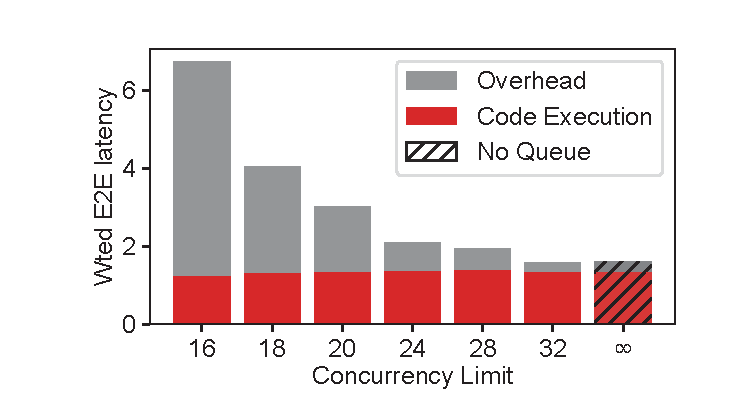
\includegraphics[width=0.6\textwidth]{iluvatar/graphs/old-baseline/breakdown/all_funcs_minheap_ed.pdf}}
  \hfill
  \subfloat[Distribution of function latencies \label{fig:q-base:box}] {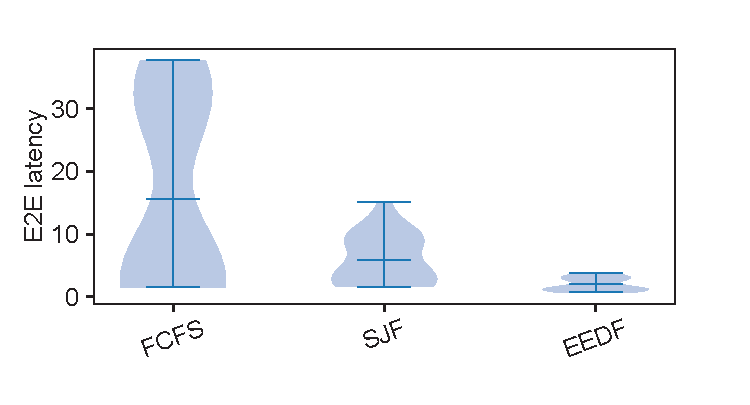
\includegraphics[width=0.6\textwidth]{iluvatar/graphs/scaled_trace2/trace_0_1/violin_e2e_for_each_queue/16_16.pdf}}
  \hfill
  \subfloat[Latency breakdown \label{fig:q-base:breakdown}] {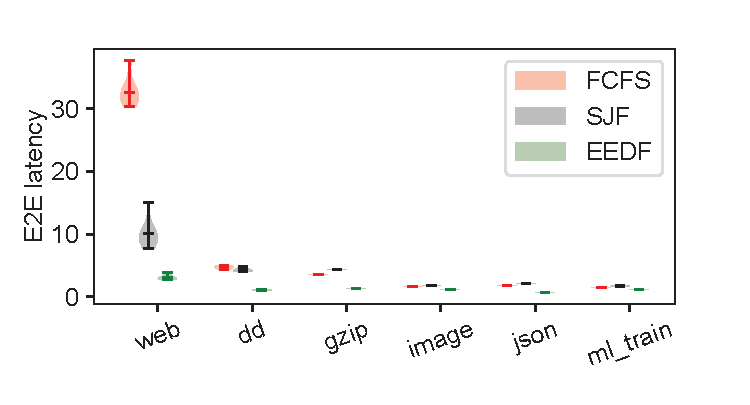
\includegraphics[width=0.6\textwidth]{iluvatar/graphs/scaled_trace2/trace_0_1/violin_func_breakdown/16_16.pdf}}
% \vspace*{-6pt}
  \caption{Queuing performance on the stationary Azure workload. Size-based policies can provide significant latency benefits.}
  \label{fig:q-baseline}
  %  \vspace*{-6pt}
\end{figure*}


\noindent \textbf{Metrics.} 
We use multiple performance metrics to understand and compare different policies.
Since functions can differ in execution time, we always normalize their total latency (flow time) by their execution time in an unloaded system. 
As shown in the previous figures~\ref{fig:flow-fn-all}, even with 1 closed-loop thread, the execution time has variance.
For normalization, we use the \emph{average} execution time with 1 thread for all the functions. 
Second, function popularities can also vary widely. 
We thus compute the \emph{weighted} latency, where each function's normalized latency is weighted by the number of its invocations in the trace.
Thus, the weighted latency represents the latency \emph{per-invocation}. 

\begin{figure}
  \centering 
  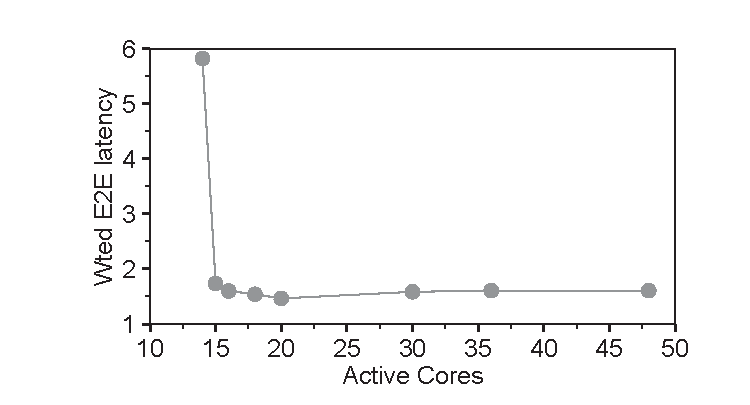
\includegraphics[width=0.6\textwidth]{iluvatar/graphs/scaling/WeakScaling.pdf}
    %  \vspace*{-6pt}
  \caption{The per-invocation function latencies for different system sizes (\# CPUs). We see a sharp inflection point at 16 CPUs, and use that in our queuing evaluation.}
    %  \vspace*{-6pt}
  \label{fig:weak}
\end{figure}


\noindent \textbf{Saturation Testing.}
We are primarily interested in how the queuing impacts the waiting time (which is part of the control plane overhead), and the function performance.
The analysis of queuing is interesting only in saturated scenarios, where there is enough extra load on the system and not all invocations can immediately run on the CPU.
We find this saturation point by weak scaling, and decreasing the number of CPU cores available to \sysname~(by disabling CPU cores using hot-unplug). 
The weighted and normalized latencies for different number of CPUs is shown in Figure~\ref{fig:weak}, which shows the performance \emph{without queuing.}
We see that for our baseline trace, increasing the number of available CPU cores has diminishing returns: the per-invocation latency doesnt benefit when CPUs are increased from 18 to 48.
However, we also see a sharp inflection point at 16 cores: decreasing the size to 14 cores results in a very high, almost $6\times$ slowdown. 
At 16 cores, our workload saturates the system, and we use this system configuration for all our queuing analysis.
We note that the alternative is to scale the workload up and run on on all 48 cores.
However, as we have shown previously through Figure~\ref{fig:flow-fn-all}, the poor hardware locality results in higher variance in the function execution times, and introduces more performance variance.
This variance often masks the control plane jitter, which is of more interest to us. 

% We evaluate our several queuing policies and compare them against a ``no-queue'' policy. 
% When there is no queue to limit concurrency, the control plane must either reject invocations when overloaded or allow resource overcommitment: namely processor sharing.
% Our system chooses the latter and will allow infinite invocations to run concurrently, so long as there is sufficient memory available, we do not overcommit memory.
% This behavior mimics how Openwhisk handles overload scenarios.
\begin{figure*}
  \centering
  \subfloat[Overcommit \label{fig:q-burst:wted}] {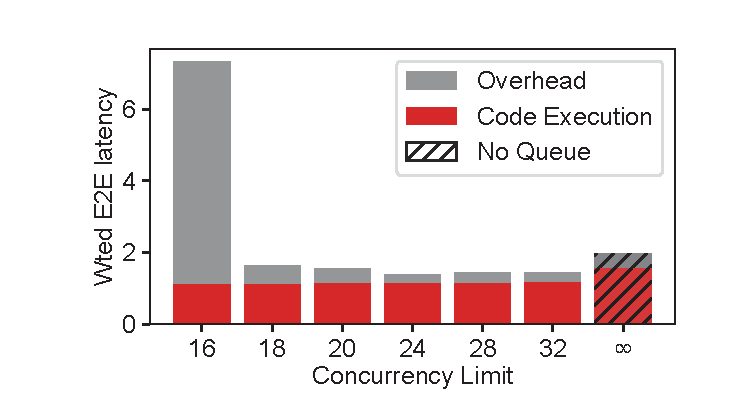
\includegraphics[width=0.6\textwidth]{iluvatar/graphs/scaled_burst_trace2/trace_0_1/barplot_breakdown_perqueue/all_funcs_minheap_ed.pdf}}
  \hfill
  \subfloat[Distribution of function latencies \label{fig:q-burst:box}] {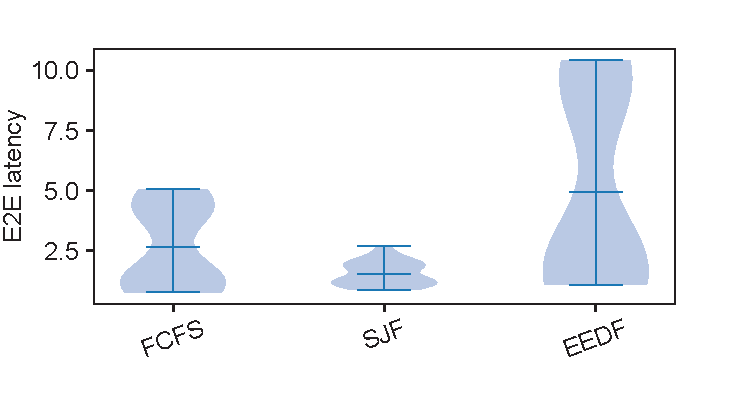
\includegraphics[width=0.6\textwidth]{iluvatar/graphs/scaled_burst_trace2/trace_0_1/violin_e2e_for_each_queue/16_16.pdf}}
  \hfill
  \subfloat[Latency Breakdown \label{fig:q-burst:breakdown}] {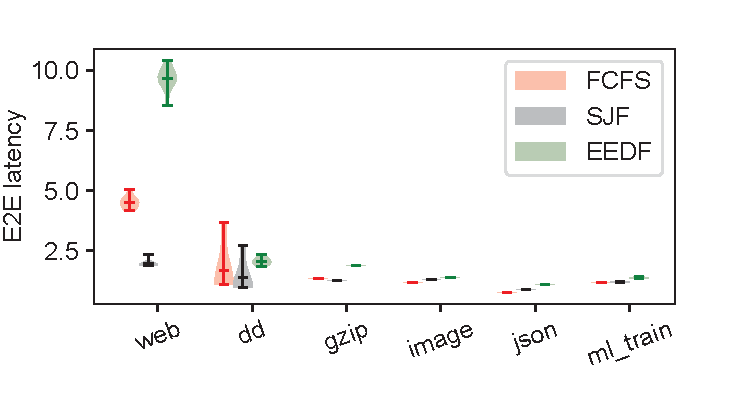
\includegraphics[width=0.6\textwidth]{iluvatar/graphs/scaled_burst_trace2/trace_0_1/violin_func_breakdown/16_16.pdf}}
    %  \vspace*{-6pt}
  \caption{Small and bursty functions can get disproportionately impacted due to queuing. A little overcommitment can go a long way to reduce latency.}
    %  \vspace*{-6pt}
  \label{fig:q-burst}
\end{figure*}

\noindent \textbf{Impact of Overcommitment.}
Many frameworks like OpenWhisk inadvertently overcommit CPUs by running more functions than available CPU cores.
\sysname~can control the degree of overcommitment through its concurrency limit queue regulator.
Figure~\ref{fig:q-base:wted} shows the effect of this overcommitment, when the EEDF (earliest effective deadline) queue policy is used. 
The worker is limited to CPU cores, so higher concurrency limits represent different degrees of overcommitment. 
As the concurrency limit is increased, we see a reduction in the queuing time (which is a major part of the control plane overhead).
For instance, the queuing overhead is negligible when overcommitment level is 2 (i.e., 32 concurrency limit).
However we can see a tradeoff: the increased concurrency risks performance interference, and the code execution time also slightly increases (by 4\%).
For comparison and as a baseline, we also show the \quotes{no queue} configuration which is pure processor sharing and there is no limit on CPU overcommitment.
%
Queuing also reduces cold starts due to concurrent invocations. 
Without queuing, the number of cold starts increased by more than $3\times$. 

For the bursty workload, the impact of overcommitment is even more drastic, as shown in Figure~\ref{fig:q-burst:wted}.
A slight increase in concurrency limit can reduce the weighted latency by more than $3\times$, indicating that overcommitment is more effective for burstier workloads.
Interestingly, the latency improves by $20\%$ with queuing as compared to the \quotes{infinite overcommitment} no queuing case.
This is due to the increase in function execution time due to uncontrolled CPU contention and interference, which the queue helps ameliorate. 

\noindent \textbf{Result:} \emph{CPU overcommitment can reduce queuing times, but come with risk of increased performance interference. \sysname's queue design provides a new effective \quotes{knob} for managing this tradeoff.}

% Bursty here. 

\noindent \textbf{Queuing Policies and Fairness.}
Next, we look at the performance impact of the different queuing policies themselves.
We are interested in the impact on the latencies of the different functions. 
Figure~\ref{fig:q-base:box} shows the normalized latencies of different functions with the different queuing policies.
This scenario has a significant amount of queuing: the concurrency limit is set to 16 (the number of CPUs). 
The function-size aware policies like SJF and EEDF provide much lower latency compared to the standard FCFS: the average latency is reduced by more than $2-3\times$. % 30 to 10 
%The RARE policy prioritizes the highest inter arrival time, and is not size aware, and also tends to suffer under high loads.

A breakdown of the latency of individual functions in Figure~\ref{fig:q-base:breakdown} helps understand this stark performance difference.
The queuing in FCFS increases the total time of the extremely small \quotes{web} function (13ms running time), which increases its latency by $30\times$.
The small-function prioritization by SJF and EEDF reduces this significantly. 

The impact of queuing for the bursty workload is even more interesting, as shown in Figure~\ref{fig:q-burst:box}.
EEDF's average latency is $2\times$ higher than simple FCFS, while SJF is 60\% lower than FCFS. 
Investigating the per-function breakdown again in Figure~\ref{fig:q-burst:breakdown} again points to the contribution of the small web function, which is \emph{also the bursty function}.
The bursty invocations trigger the cold start mitigation, which deprioritizes them, and increases the queuing time, which disproportionately impacts the small functions.
% Bursty here. 

\noindent \textbf{Result:} \emph{Incorporating both function size and arrival times can improve function latency and fairness significantly. Very small functions see a higher \% increase due to queuing.}


%%%%%%%%%%%%%%%%%%%%%%%%%%%%%%


\noindent \textbf{\sysname~vs. Little's law vs. Simulation.}
Finally, we want to show \sysname's suitability for performance modeling, capacity planning, and as a research control plane for developing and evaluating FaaS resource management policies.
We compare the number of concurrent function invocations and queue length (EEDF) with the expected load according to Little's law, computed using average arrival rates and execution times of all functions of our stationary trace. 
We see that the real system metrics, even with all the inherent burstiness in the Azure trace, and the function execution and control plane jitter, are on average very close to the Little's law estimate.
This strongly indicates that our performance is indeed predictable even with highly heterogeneous workloads.

Additionally, Figure~\ref{fig:sim-vs-live-little} also shows the output of our ``simulation'' container backend described in Section~\ref{sec:design:ctr}.
This backend doesn't run actual function code, but exercises all other control plane aspects.
We use constant average function execution times (without accounting for variance and stochasticity) for all invocations.
Even though this simulation setup doesn't capture real-world variability and the impact of server load on function performance, we see that the simulation is also fairly closely aligned with the real experiment output.
This shows that \sysname's integrated simulation framework captures sufficient system dynamics and provides high-fidelity simulations.
This can significantly accelerate FaaS research, especially advances in reinforcement learning based scheduling, which requires high-quality simulations for learning policies. 

\begin{figure}
  \centering
  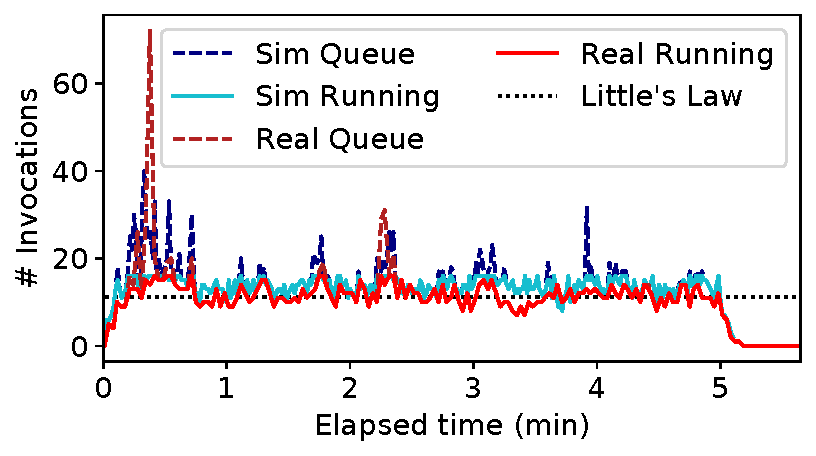
\includegraphics[width=0.6\textwidth]{iluvatar/graphs/trace-compare/baseline/minheap_ed/16/paper-status.pdf}
  \caption{\sysname~running in-silico closely models the in-situ performance. Making it a viable exploration opportunity supplementing real experiments.}
  \label{fig:sim-vs-live-little}
\end{figure}

% \subsection{Scalability}
% \label{sec:eval:scale}

% \textbf{Strong scaling. 48 worse than 16 because of ... bad locality?}

% \textbf{Simulation.}
% FaaS performance highly sensitive to workload due to skewed nature.
% Tough to experiment and report stable outcomes.
% For example, adding one function \emph{decreases} the overall latency. But its due to reporting.

% One way to avoid this is to look into simulations. Lightweight and allow different combinations to be thoroughly explored.

\begin{comment}
\noindent \textbf{Discussion.}
Our worker-centric design allows us to focus on single-worker performance. 
The load balancer is stateless and uses consistent hashing with bounded loads, and has a small overhead of less than 0.5 ms. 
Without workers sharing state (like with OpenWhisk's shared queue), there is no/minimal performance interference, and hotspots are confined in space and time.
%We conjecture that \sysname's performance improvements are largely due to the design and queuing policies for handling invocation bursts. 

Finally, our performance comparison with OpenWhisk is based on end-to-end latency testing. 
Performance tracing of OpenWhisk is challenging due to the highly distributed nature, and the drastically different architectures prevent a clean side-by-side comparison vs. the various components.
The use of Rust vs. Scala provides some performance gains as well, but all our OpenWhisk evaluation was conducted with ample heap sizes to reduce extra garbage collection overheads. 
\end{comment}

\begin{comment}
\begin{figure*}
  \centering
  \subfloat[Overcommit \label{fig:q-base:wted}] {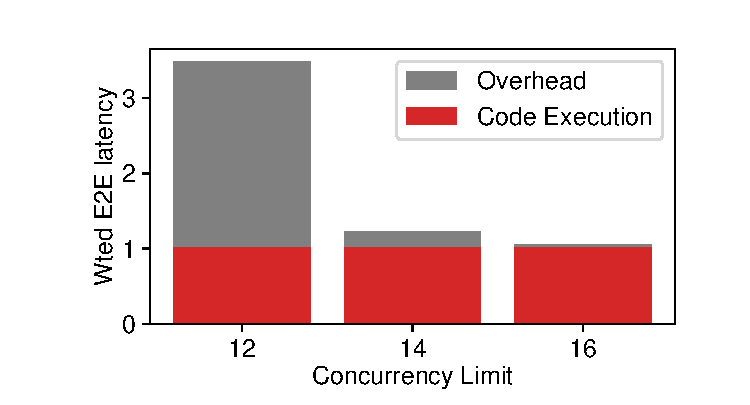
\includegraphics[width=0.3\textwidth]{iluvatar/graphs/simulation/scaled_trace2/trace_0_1/barplot_breakdown_perqueue/all_funcs_minheap_ed.pdf}}
  \hfill
  \subfloat[Distribution of function latencies \label{fig:q-base:box}] {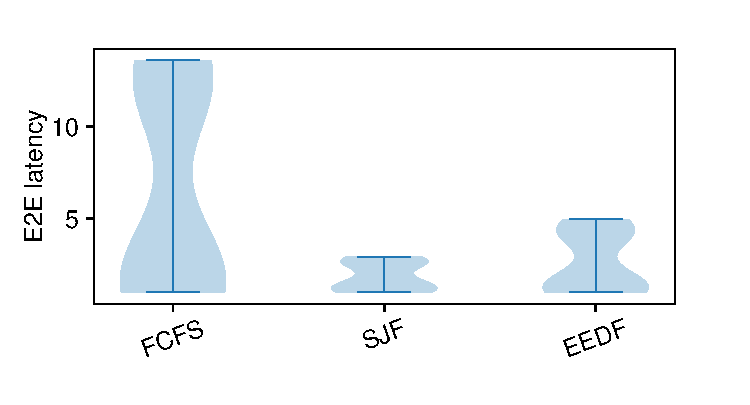
\includegraphics[width=0.3\textwidth]{iluvatar/graphs/simulation/scaled_trace2/trace_0_1/violin_e2e_for_each_queue/16_12.pdf}}
  \hfill
  \subfloat[Code Breakdown \label{fig:q-base:cold}] {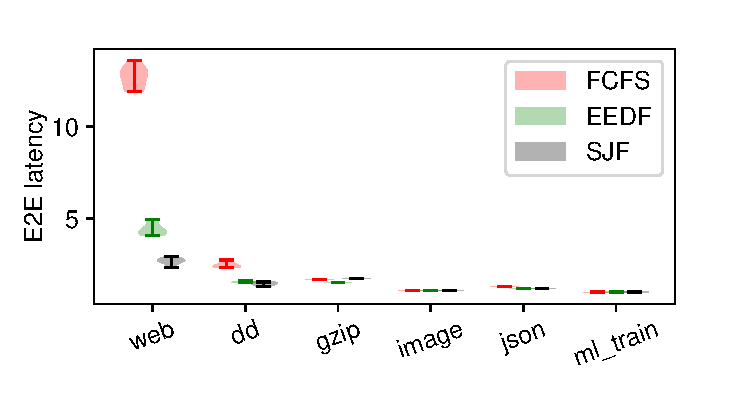
\includegraphics[width=0.3\textwidth]{iluvatar/graphs/simulation/scaled_trace2/trace_0_1/violin_func_breakdown/16_12.pdf}}
 
  % \subfloat[Overcommit \label{fig:q-base:wted}] {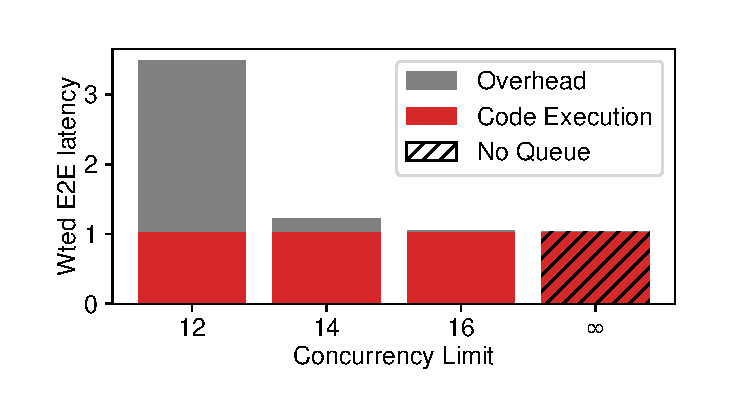
\includegraphics[width=0.3\textwidth]{iluvatar/graphs/burst/breakdown/all_funcs_minheap_ed.pdf}}
  % \hfill
  % \subfloat[Fairness \label{fig:q-base:box}] {\includegraphics[width=0.3\textwidth]{iluvatar/graphs/burst/boxplot/16_24.pdf}}
  % \hfill
  % \subfloat[Cold \label{fig:q-base:cold}] {\includegraphics[width=0.3\textwidth]{iluvatar/graphs/burst/coldstarts/16_24.pdf}}
    % \vspace*{-6pt}
  \caption{Simulation baseline}
  \label{fig:q-burst}
    %  \vspace*{-6pt}
\end{figure*}
\end{comment}

%%% Local Variables:
%%% mode: latex
%%% TeX-master: "paper"
%%% End:


\section{Related Work}
\label{sec:related}

Alongside the closed-source FaaS control planes from the major cloud providers, a variety of other FaaS control planes exist.
Open-source production faas OpenWhisk~\cite{openwhisk}, OpenFaaS~\cite{openfaas}, nuclio~\cite{nuclio}, kNative~\cite{knative}, and funcX~\cite{funcx_hpdc_20}.
Others were made for with targeted research goals in mind~\cite{jia2021nightcore, hendrickson2016serverless, oakes_sock_2018, singhvi2021atoll,vhive-asplos21}.

\sysname~occupies a somewhat unique spot in the crowded FaaS landscape because of its focus on warm starts and some key constraints in our system design.
%
Techniques for reducing cold start overheads, like snapshots, language isolation,  unikernels, all sit ``below'' the control plane, and can be complemented with fast control planes.
At the other extreme end, the predictable nature of serverless workloads has been used to great effect for predictive load-balancing, prefetching, sizing, etc.
\sysname~is mostly reactive and is worker-centric, and tries to make minimal assumptions about workload predictability and focuses on more general optimizations that can work for arbitrary workload patterns.
%

\noindent \textbf{FaaS Control Planes.}
%
SOCK~\cite{oakes_sock_2018} is closely related to \sysname, and makes similar observations about network namespace overheads, and introduced storage and cgroup optimizations for serverless optimized containers. 
SOCK is based on OpenLambda~\cite{hendrickson2016serverless} and achieves great cold start performance with Zygotes that are cloned into new containers.
These optimizations to the container runtime are also applicable to \sysname~and are complementary. 
Using the standard containerd interface allows us to use multiple current and future container backends, and is a deliberate tradeoff. 
%Importantly it lacks both the ability to operate as a cluster and an integrated load generation system, both of which we have implemented both in \sysname~.


Nightcore~\cite{jia2021nightcore} is an integrated control plane and runtime system for low-latency microsecond-scale microservices.
It essentially implements containerized RPC, and uses fast message passing between the control plane and the agent.
Its special container runtime precludes generic ``black box'' functions, and it provides a weaker isolation model by running functions concurrently within the same container.
In the microservice context, container management and scheduling, dealing with heterogenenous functions, and other challenges are not relevant.


Atoll~\cite{singhvi2021atoll} is a fast and highly scalable control plane, and hugely benefits from pre-allocation and prediction.
It has a two level load-balancing setup with functions scheduled to a cluster group which then places them on a worker. 
\sysname's design and contributions are orthogonal to Atoll's more top-down and predictive approach, and we focus on the ``low-level'' worker problems.


Open-source control planes like OpenWhisk, OpenFaaS~\cite{openfaas}, nuclio~\cite{nuclio}, and kNative~\cite{knative}, are widely used to provide functions as a service. 
They tackle the competing demands of modularity and features, along with supporting function executions in generic environments.
Many FaaS systems use Kubernetes as the resource and container management layer, and its complexity and high latency further inhibits deep understanding and optimizations. 
OpenWhisk's cold and warm performance has been analyzed in many prior works such as~\cite{quevedo_evaluating_2019} and also as part of other systems~\cite{scheuner_lets_2022, alzayat_groundhog_2022, faaslb-hpdc22, faascache-asplos21}. 
OpenWhisk scheduling design and improvements can be found in ~\cite{kim_scheduling_2021, faaslb-hpdc22}.
Tighter latency requirements exist when deploying functions at the edge, and OpenWhisk's use on lower powered devices presents even more latency troubles~\cite{palade-edge-22, pfandzelter_tinyfaas_2020, hall_execution_2019, wang2021lass}. 
Interestingly, public cloud latencies are also significant, of the order of 50 ms~\cite{ustiugov_analyzing_2021}, hinting that the problems also extend their control planes. 
%All four of these control planes rely on Docker and Kubernetes for their deployment and scaling mechanisms.
%These existing tech stacks are highly useful, but limit the research possibilities of a platform, e.g. cold start optimizations and deploying to edge nodes become intractable.
%While \sysname~does have a Docker isolation implementation, it is to showcase the ability implement multiple containerization mechanisms and compare between them.


\noindent \textbf{Function Scheduling.}
Concurrent to our efforts, queuing of function invocations has been proposed in~\cite{zuk_call_2022}, which implements various size-aware policies like SJF. 
Surprisingly, and perhaps due to OpenWhisk overheads, their function slowdowns are extremely high: of more than $10,000\times$. 
An earlier theoretical queuing analysis of flow and stretch metrics is also presented in~\cite{zuk_scheduling_2020}. 
In contrast to \sysname's worker-centric design, a centralized core-level allocation design is presented in~\cite{kaffes_centralized_2019}.
In FaaS clusters, the tradeoffs in load balancing and early/late binding are evaluated in~\cite{kaffes_hermod_2022}.
Locality~\cite{faaslb-hpdc22}  and ML-based~\cite{yu2021faasrank} techniques for FaaS load-balancing take advantage of the high temporal locality and predictability of the FaaS workloads.
Our effort is more focused on reactive systems, and adding predictive allocation will only improve it. 

OS scheduler improvements can also improve FaaS workloads~\cite{fu2022sfs}. 
Regulating Linux CPU cgroups shares is also effective in overcommitment~\cite{ensure-faas-acsos20}.
Evaluating the effectiveness of these scheduling improvements when juxtaposed with queuing will be interesting. 
Scheduling function workflows and DAGs are a growing area~\cite{shen_defuse_2021,mahgoub_wisefuse_2022,zhou_qos-aware_2022}, and we focus on single-invocation optimizations. 

\begin{comment}
Restoring from snapshots~\cite{vhive, faasnap, catalyzer}


%The architectural implications are analyzed in~\cite{shahrad_architectural_2019}. We look at the higher levels of the stack, i.e., at the control plane. The paper identifies the fundamental factors affecting function performance at the hardware level due to cache misses, bad locality, etc. 
\paragraph{Edge.}
The lower resource availability of edge platforms also motivates lighter control planes. 
Tinyfaas is a apecialized FaaS platform for the edge 
\cite{pfandzelter_tinyfaas_2020}, but uses existing control planes like OpenWhisk and Kubless.
\cite{hall_execution_2019}


\paragraph{Scheduling.}

ANY papers that use previous running time/task size information!? Atoll. Aquatope. 

Tail latency: 50ms for warm-starts for the cloud.~\cite{ustiugov_analyzing_2021} 

RL scheduling~\cite{yu2021faasrank}. 

Lets trace it\cite{scheuner_lets_2022} , platform overheads etc.


Workflow and serverless DAG scheduling is complementary to \sysname. 

FnSched. Anshul~\cite{}. Centralized Scheduling? 

Sharing containers in SAND~\cite{akkus_sand_2018}

Hierarchical scheduling (within container) in HyperFaas. 

\paragraph{OpenWhisk.}
\cite{quevedo_evaluating_2019} evaluates the cold and warm times under OpenWhisk. 
OW Hash based scheduling described in~\cite{kim_scheduling_2021}.

Container sizing lot of attention, why! Uses OpenWhisk atleast\cite{guo_decomposing_2022}.
Also uses it and claims massive speedups.~\cite{kotni2021faastlane}

Aquatope\cite{zhou_qos-aware_2022} also uses prewarming for keepalive and is based on OpenWhisk.

%%%%%%%%%

Overcommittment: Owl~\cite{tian_owl_2022} also does interference.
So does ENSURE and fnsched. Overcommittment has impact on both the function execution time and control plane overhead (more functions to execute and more contention of cplane processes with functions.) We do overcommitment for only short functions with the bypass. Longer functions likely to be CPU intensive.


Our work: control plane sandwiched between isolation optimizations and data-driven overcommit and predictive. 

Completely orthogonal to optimal sizing like sizeless~\cite{}, OFC~\cite{}, COSE~\cite{akhtar_cose_2020},~\cite{guo_decomposing_2022}, etc.
\end{comment}

